\documentclass[ignorenonframetext,]{beamer}
\setbeamertemplate{caption}[numbered]
\setbeamertemplate{caption label separator}{: }
\setbeamercolor{caption name}{fg=normal text.fg}
\beamertemplatenavigationsymbolsempty
\usepackage{lmodern}
\usepackage{amssymb,amsmath}
\usepackage{ifxetex,ifluatex}
\usepackage{fixltx2e} % provides \textsubscript
\ifnum 0\ifxetex 1\fi\ifluatex 1\fi=0 % if pdftex
\usepackage[T1]{fontenc}
\usepackage[utf8]{inputenc}
\else % if luatex or xelatex
\ifxetex
\usepackage{mathspec}
\else
\usepackage{fontspec}
\fi
\defaultfontfeatures{Ligatures=TeX,Scale=MatchLowercase}
\fi
\usetheme{Singapore}
% use upquote if available, for straight quotes in verbatim environments
\IfFileExists{upquote.sty}{\usepackage{upquote}}{}
% use microtype if available
\IfFileExists{microtype.sty}{%
\usepackage{microtype}
\UseMicrotypeSet[protrusion]{basicmath} % disable protrusion for tt fonts
}{}
\newif\ifbibliography
\usepackage{graphicx,grffile}
\makeatletter
\def\maxwidth{\ifdim\Gin@nat@width>\linewidth\linewidth\else\Gin@nat@width\fi}
\def\maxheight{\ifdim\Gin@nat@height>\textheight0.8\textheight\else\Gin@nat@height\fi}
\makeatother
% Scale images if necessary, so that they will not overflow the page
% margins by default, and it is still possible to overwrite the defaults
% using explicit options in \includegraphics[width, height, ...]{}
\setkeys{Gin}{width=\maxwidth,height=\maxheight,keepaspectratio}

% Prevent slide breaks in the middle of a paragraph:
\widowpenalties 1 10000
\raggedbottom

\AtBeginPart{
\let\insertpartnumber\relax
\let\partname\relax
\frame{\partpage}
}
\AtBeginSection{
\ifbibliography
\else
\let\insertsectionnumber\relax
\let\sectionname\relax
\frame{\sectionpage}
\fi
}
\AtBeginSubsection{
\let\insertsubsectionnumber\relax
\let\subsectionname\relax
\frame{\subsectionpage}
}

\setlength{\parindent}{0pt}
\setlength{\parskip}{6pt plus 2pt minus 1pt}
\setlength{\emergencystretch}{3em}  % prevent overfull lines
\providecommand{\tightlist}{%
\setlength{\itemsep}{0pt}\setlength{\parskip}{0pt}}
\setcounter{secnumdepth}{0}
\usepackage{graphicx}
\usepackage{array}
\usepackage{tabularx}                                             % table environment providing flexibility
\usepackage{caption}                                              % for creating captions  
\usepackage{longtable}                                            % allows tables to span multiple pages
\usepackage{rotating}                                             % allows for sideways tables
%\usepackage{float}                                                % floating environments; may not need in rmarkdown
%\usepackage{placeins}                                             % keeps floats from moving
%\usepackage{indentfirst}                                          % indents first paragraph of a section
%\usepackage{mdwtab}                                               % continued float multi-page figure
\usepackage{enumerate}                                            % create lists
\usepackage{hyperref}                                             % highlight cross references
\usepackage{enumitem}                                             % numbered lists
%\usepackage{upquote}                                              % produce grave accent in latex
\usepackage{verbatim}                                             % produces verbatim results
\usepackage{fancyvrb}                                             % verbatim in a box
%\usepackage{textcomp}                                             % fixes error with packages interfering
%\usepackage{cmap}                                                 % fix mapping characters to unicode
\usepackage{lscape}

\setbeamersize{text margin left=0.2in}
\setbeamersize{text margin right=0.2in}

\definecolor{pageCol}{rgb}{0.5,0.5,1.0}

\usepackage{tikz}                                                   % used in background


\usebackgroundtemplate{
  \tikz[overlay,remember picture] 
  \node[opacity=0.3, at=(current page.south east),anchor=south east,inner sep=0pt] {
    
\includegraphics[height=0.5in]{noaalogo.jpg}};
}

\setbeamertemplate{footline}
{
  \begin{beamercolorbox}[wd=.05\paperwidth,ht=0ex,dp=0ex,left]{framenumber in head/foot}%
    \insertframenumber/\inserttotalframenumber
    
  \end{beamercolorbox}%
}
\setbeamercolor{footline}{fg=pageCol}


\newcounter{saveenumi}

%Itemize with bullet
\setbeamertemplate{itemize item}{$\circ$}

%To get two columns
\def\begincols{\begin{columns}}
\def\begincol{\begin{column}}
\def\endcol{\end{column}}
\def\endcols{\end{columns}}


%Remove section and subsection slides
\AtBeginSubsection{}
\AtBeginSection{}

\title{California Scorpionfish 2017 Stock Assessment}
\author{Melissa H Monk\(^1\), \and Xi He\(^1\), \and John Budrick\(^2\)}
\institute{\(^1\)Southwest Fisheries Science Center \and \(^2\)California Department of Fish and Wildlife}
\date{SSC Groundfish subcommittee August 28, 2017}

\begin{document}
\frame{\titlepage}

\begin{frame}
\tableofcontents[hideallsubsections]
\end{frame}

\begin{frame}{California scorpionfish (\emph{Scorpaena guttata})}

\begin{itemize} 
 \item[$\bullet$] Most common species of \emph{Scorpaena} on the U.S. West Coast, more species in Mexico
 \item[$\bullet$] Venomous dorsal, anal and pelvic spines
 \item[$\bullet$] Demersal, found over both hard and soft bottom (anectodtal evidence sugggests they prefer \emph{new} structure)
 \item[$\bullet$] Exhibit aggregating behavior (spawning and non-spawning aggregations)  
\end{itemize}

\centering
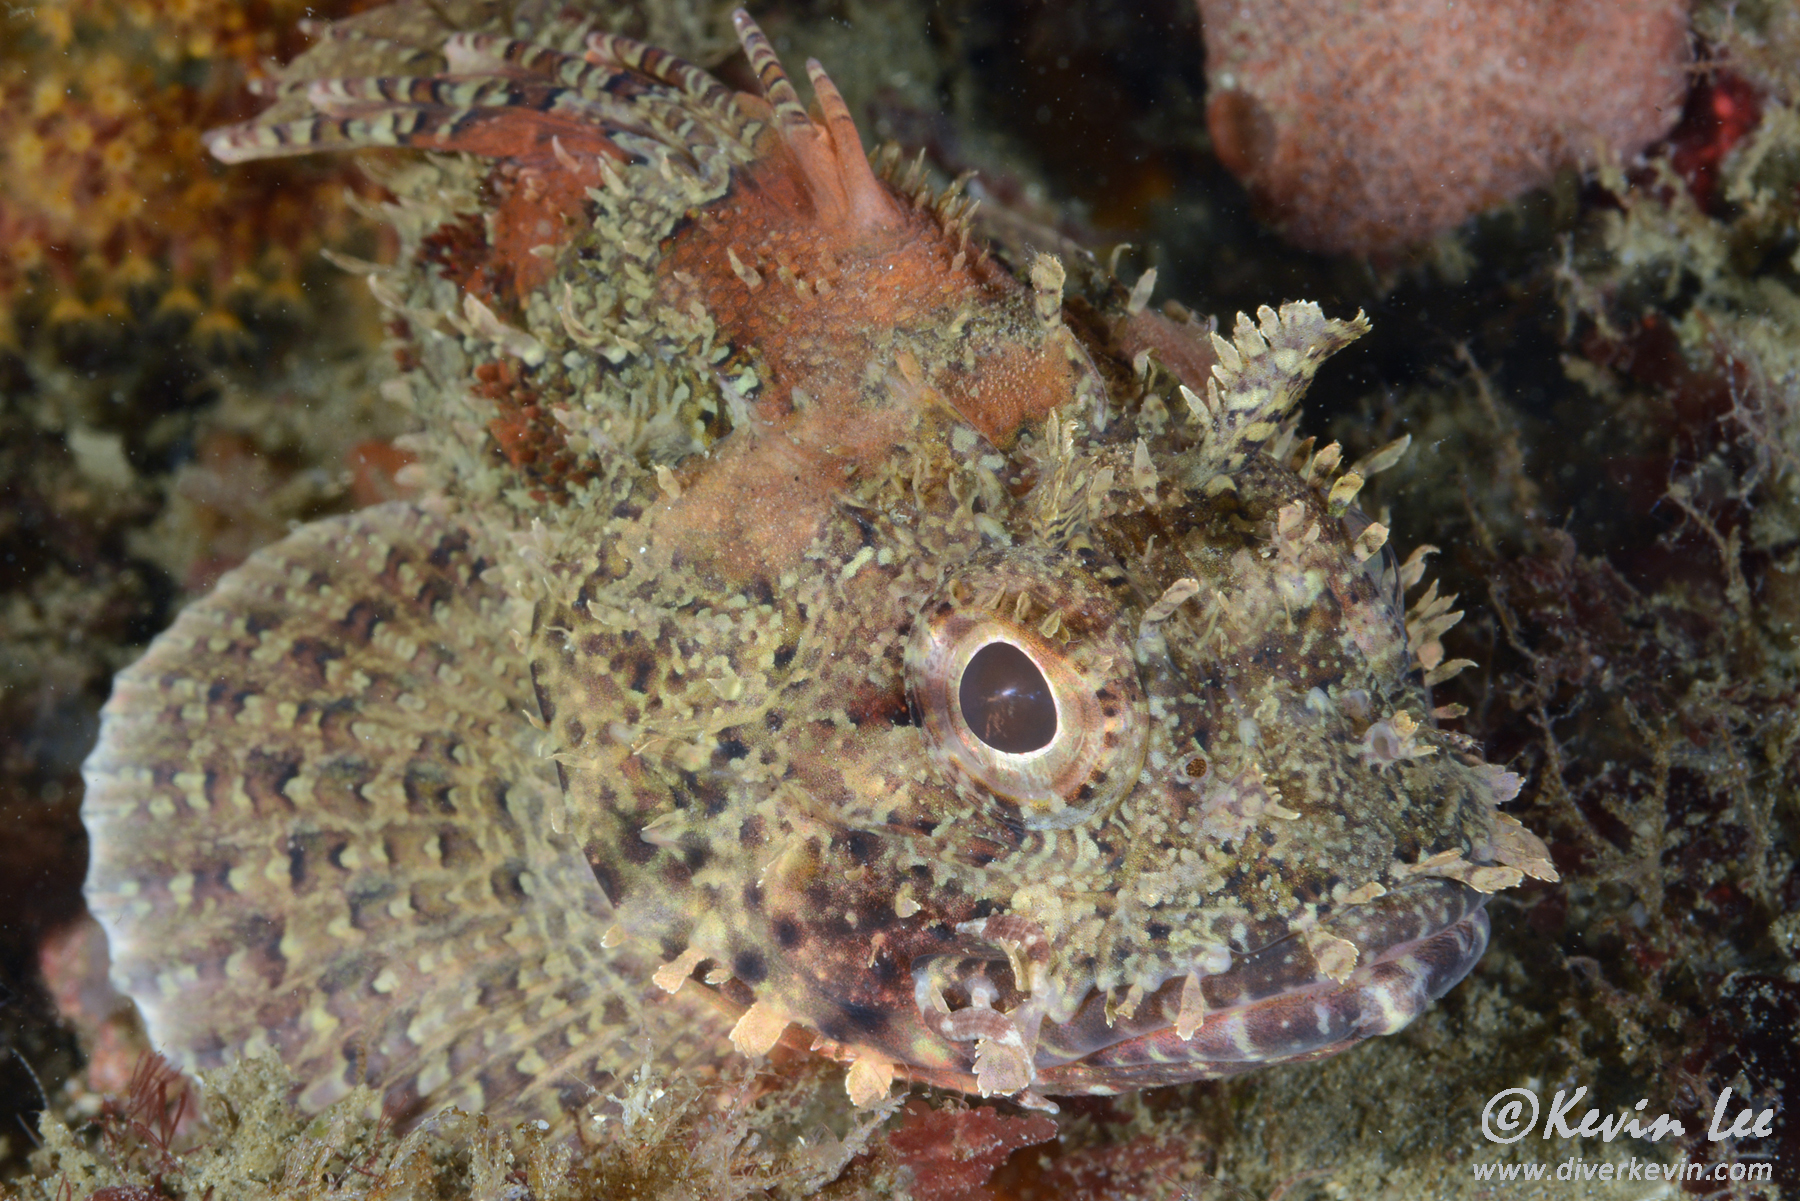
\includegraphics[width=.5\textwidth]{cover_photo}

\end{frame}

\begin{frame}{Distribution and Stock Assessment Boundary}

\begincols
 \begincol{.45\textwidth}
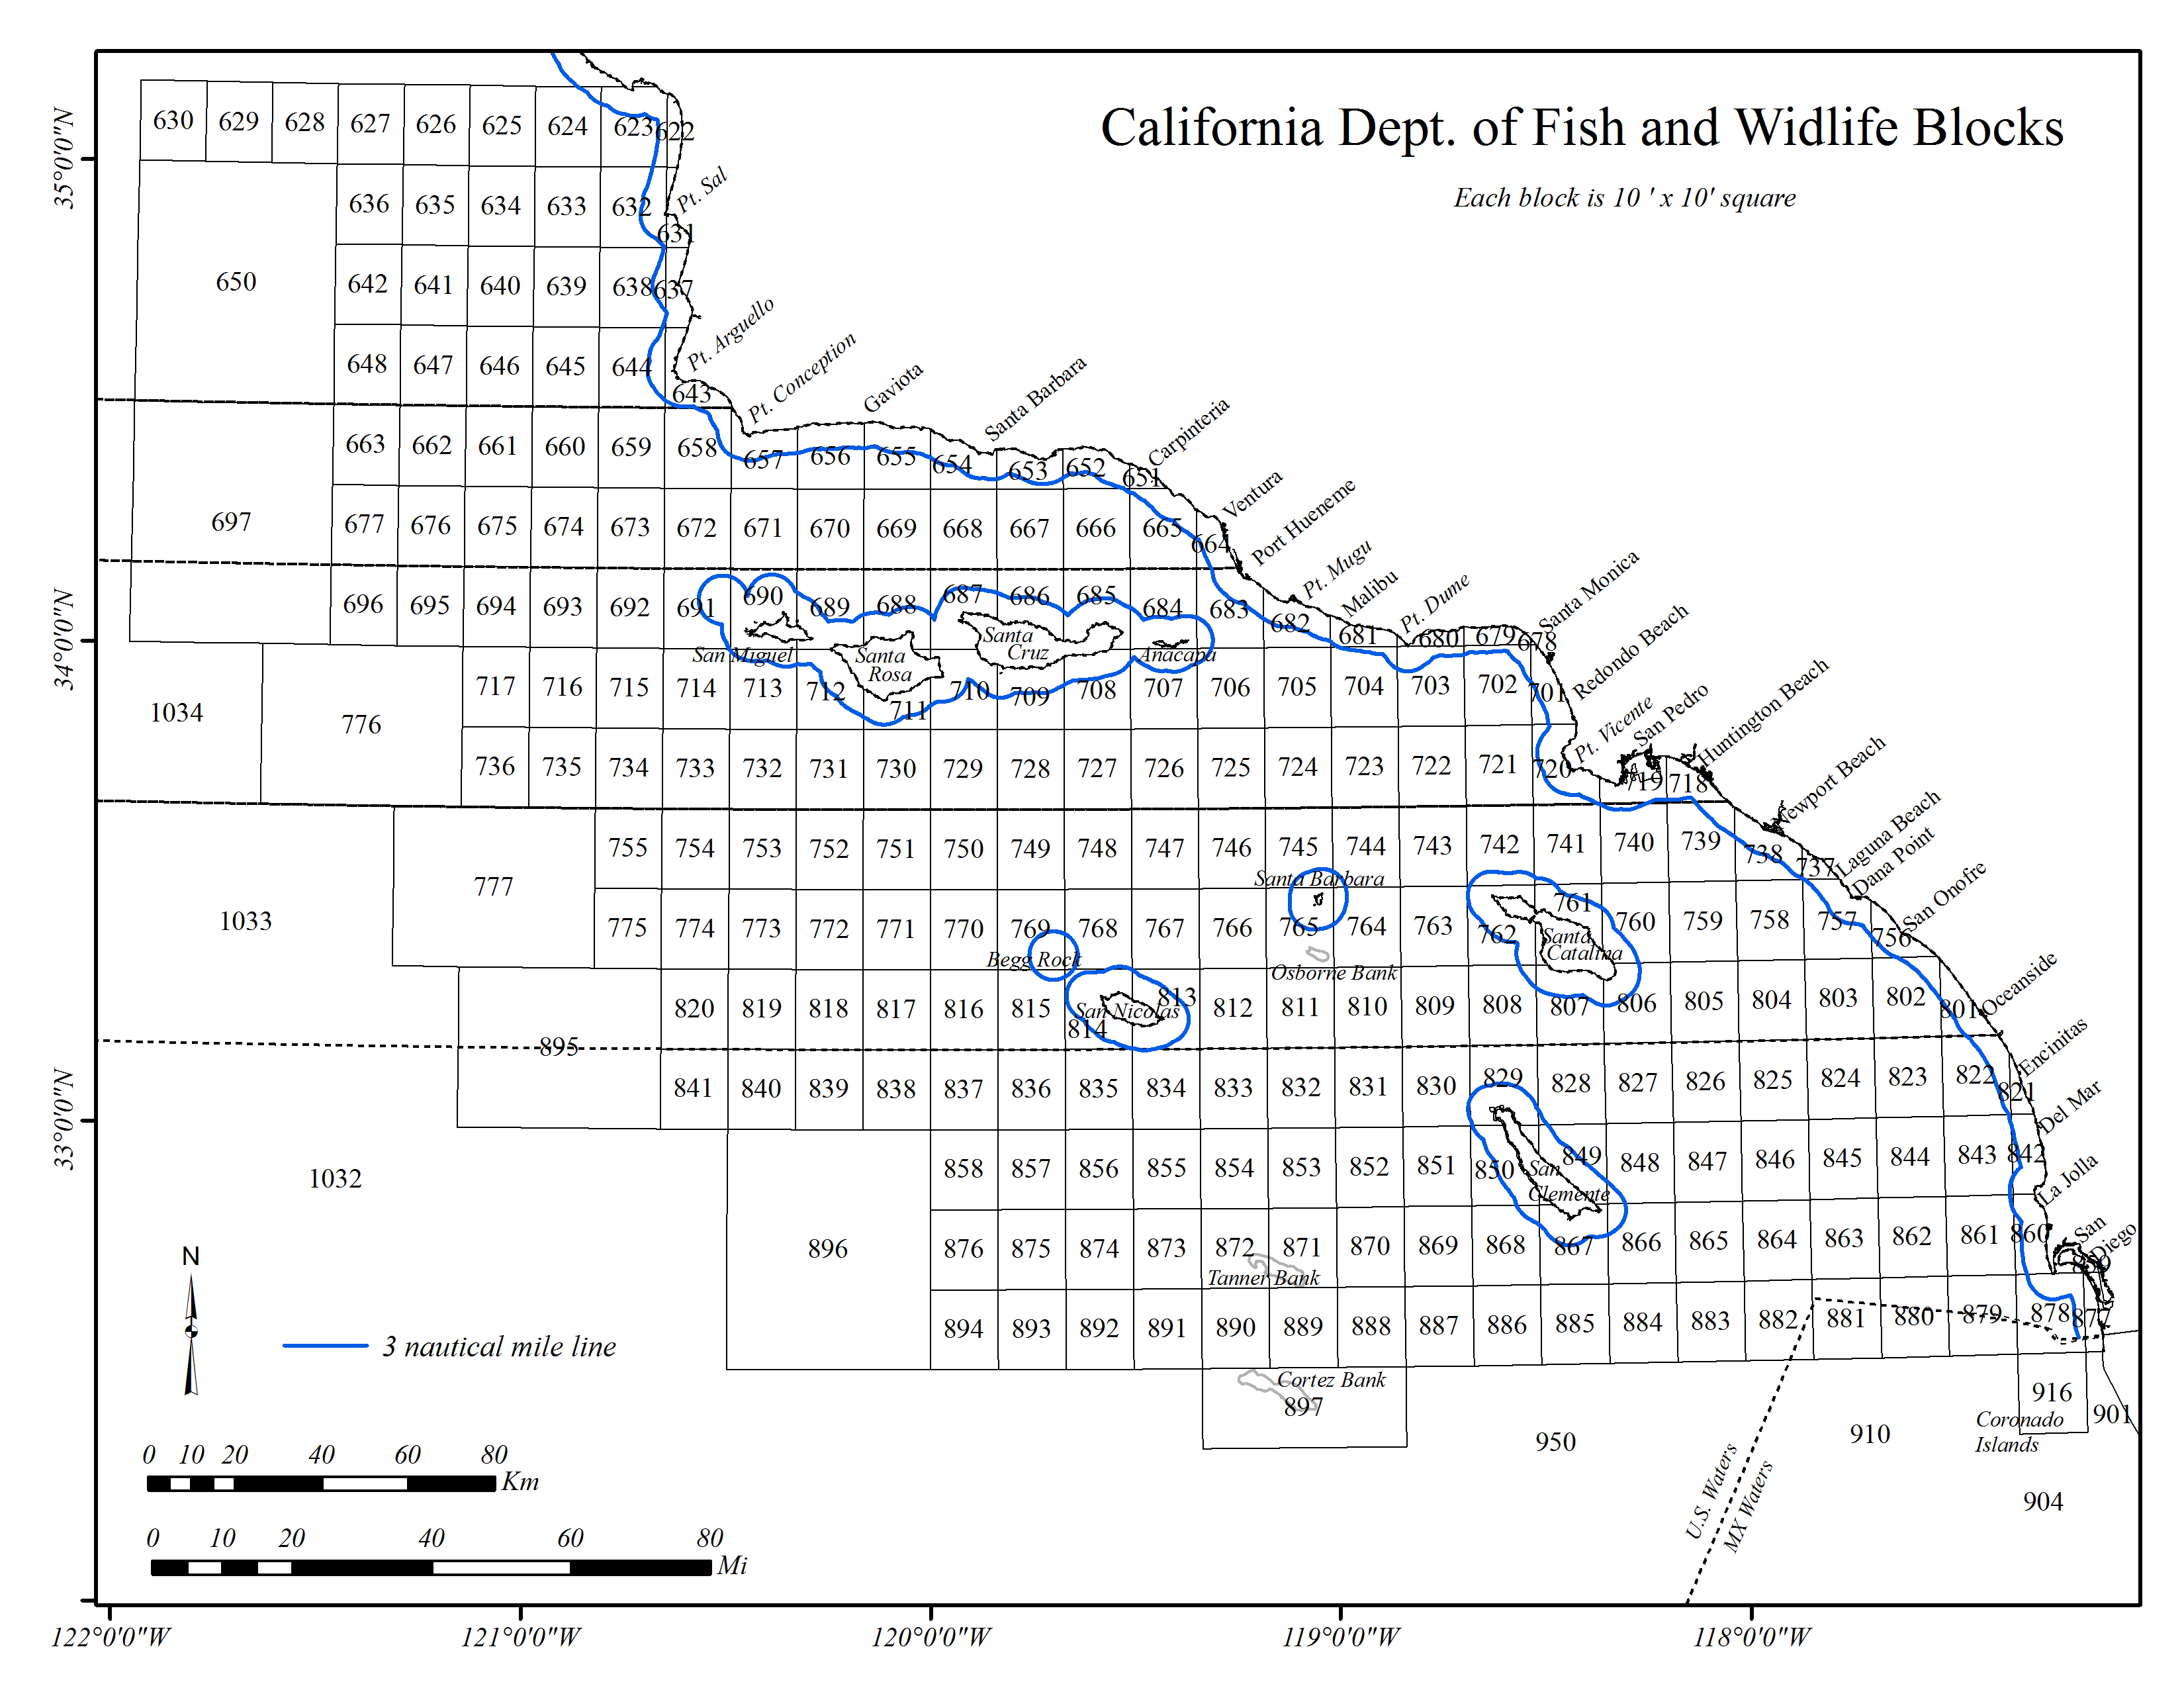
\includegraphics{Figures/assess_region_map.png}

\endcol
 \begincol{.55\textwidth}

\begin{itemize} 
 \item[$\bullet$] Distributed from central California to Punta Eugenia, Baja California Sur, Mexico 
 \item[$\bullet$] Assessment south of Pt. Conception to U.S/Mexico border 
 \item[$\bullet$] Observed from the intertidal to 600 ft,  prefer depths of 20-450 ft  
 \item[$\bullet$] Proportion of the stock in Mexican waters unknown
\end{itemize}

\endcol
\endcols

\end{frame}

\begin{frame}{Assessment History}

\begin{itemize}
\item[$\bullet$] Firt full assessment in 2005, catch-only update in 2014
\item[$\bullet$] Not all of the recreational catch was removed in the 2005 model
\item[$\bullet$] Input vs. estimated catch was not standard output in SS v.1.8
\item[$\bullet$] Catch-only update also used SS v.1.8
\end{itemize}

\begincols
 \begincol{.5\textwidth}

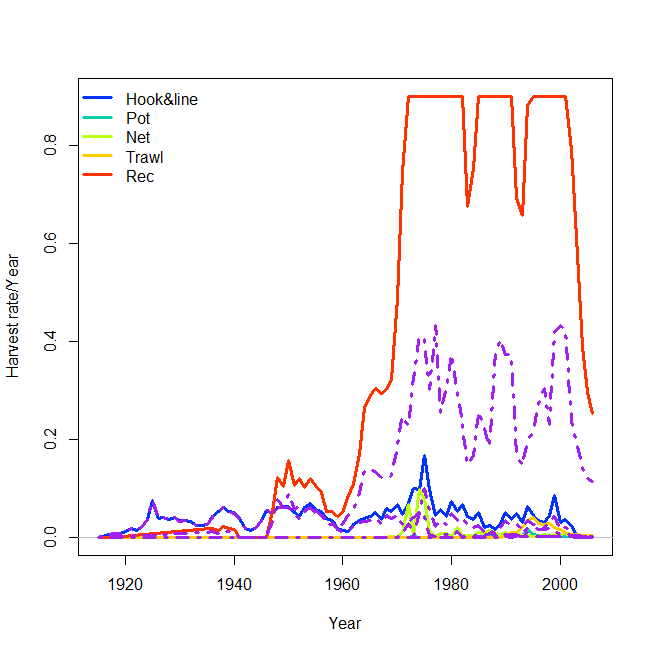
\includegraphics{Figures/bridge_harvestrate.png}

\endcol
 \begincol{.5\textwidth}

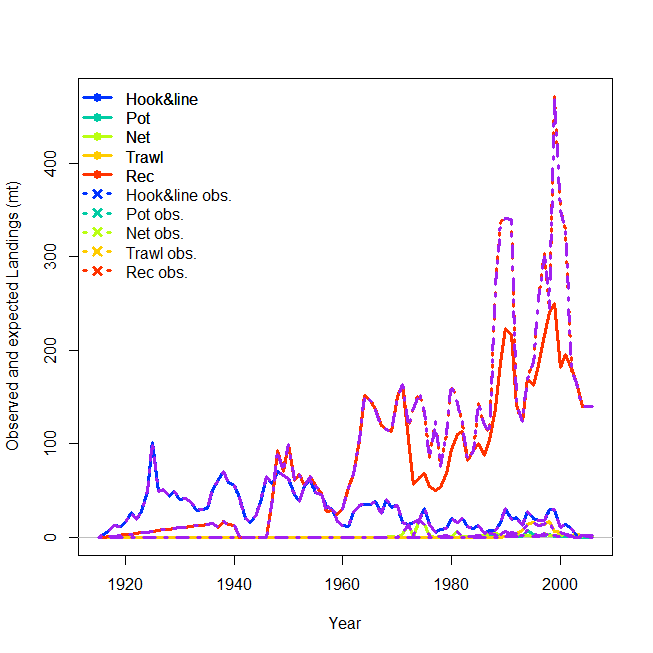
\includegraphics{Figures/bridge_catch.png}

\endcol
\endcols

\end{frame}

\begin{frame}{2017 Assessment: Catches by Fleet}

\centering
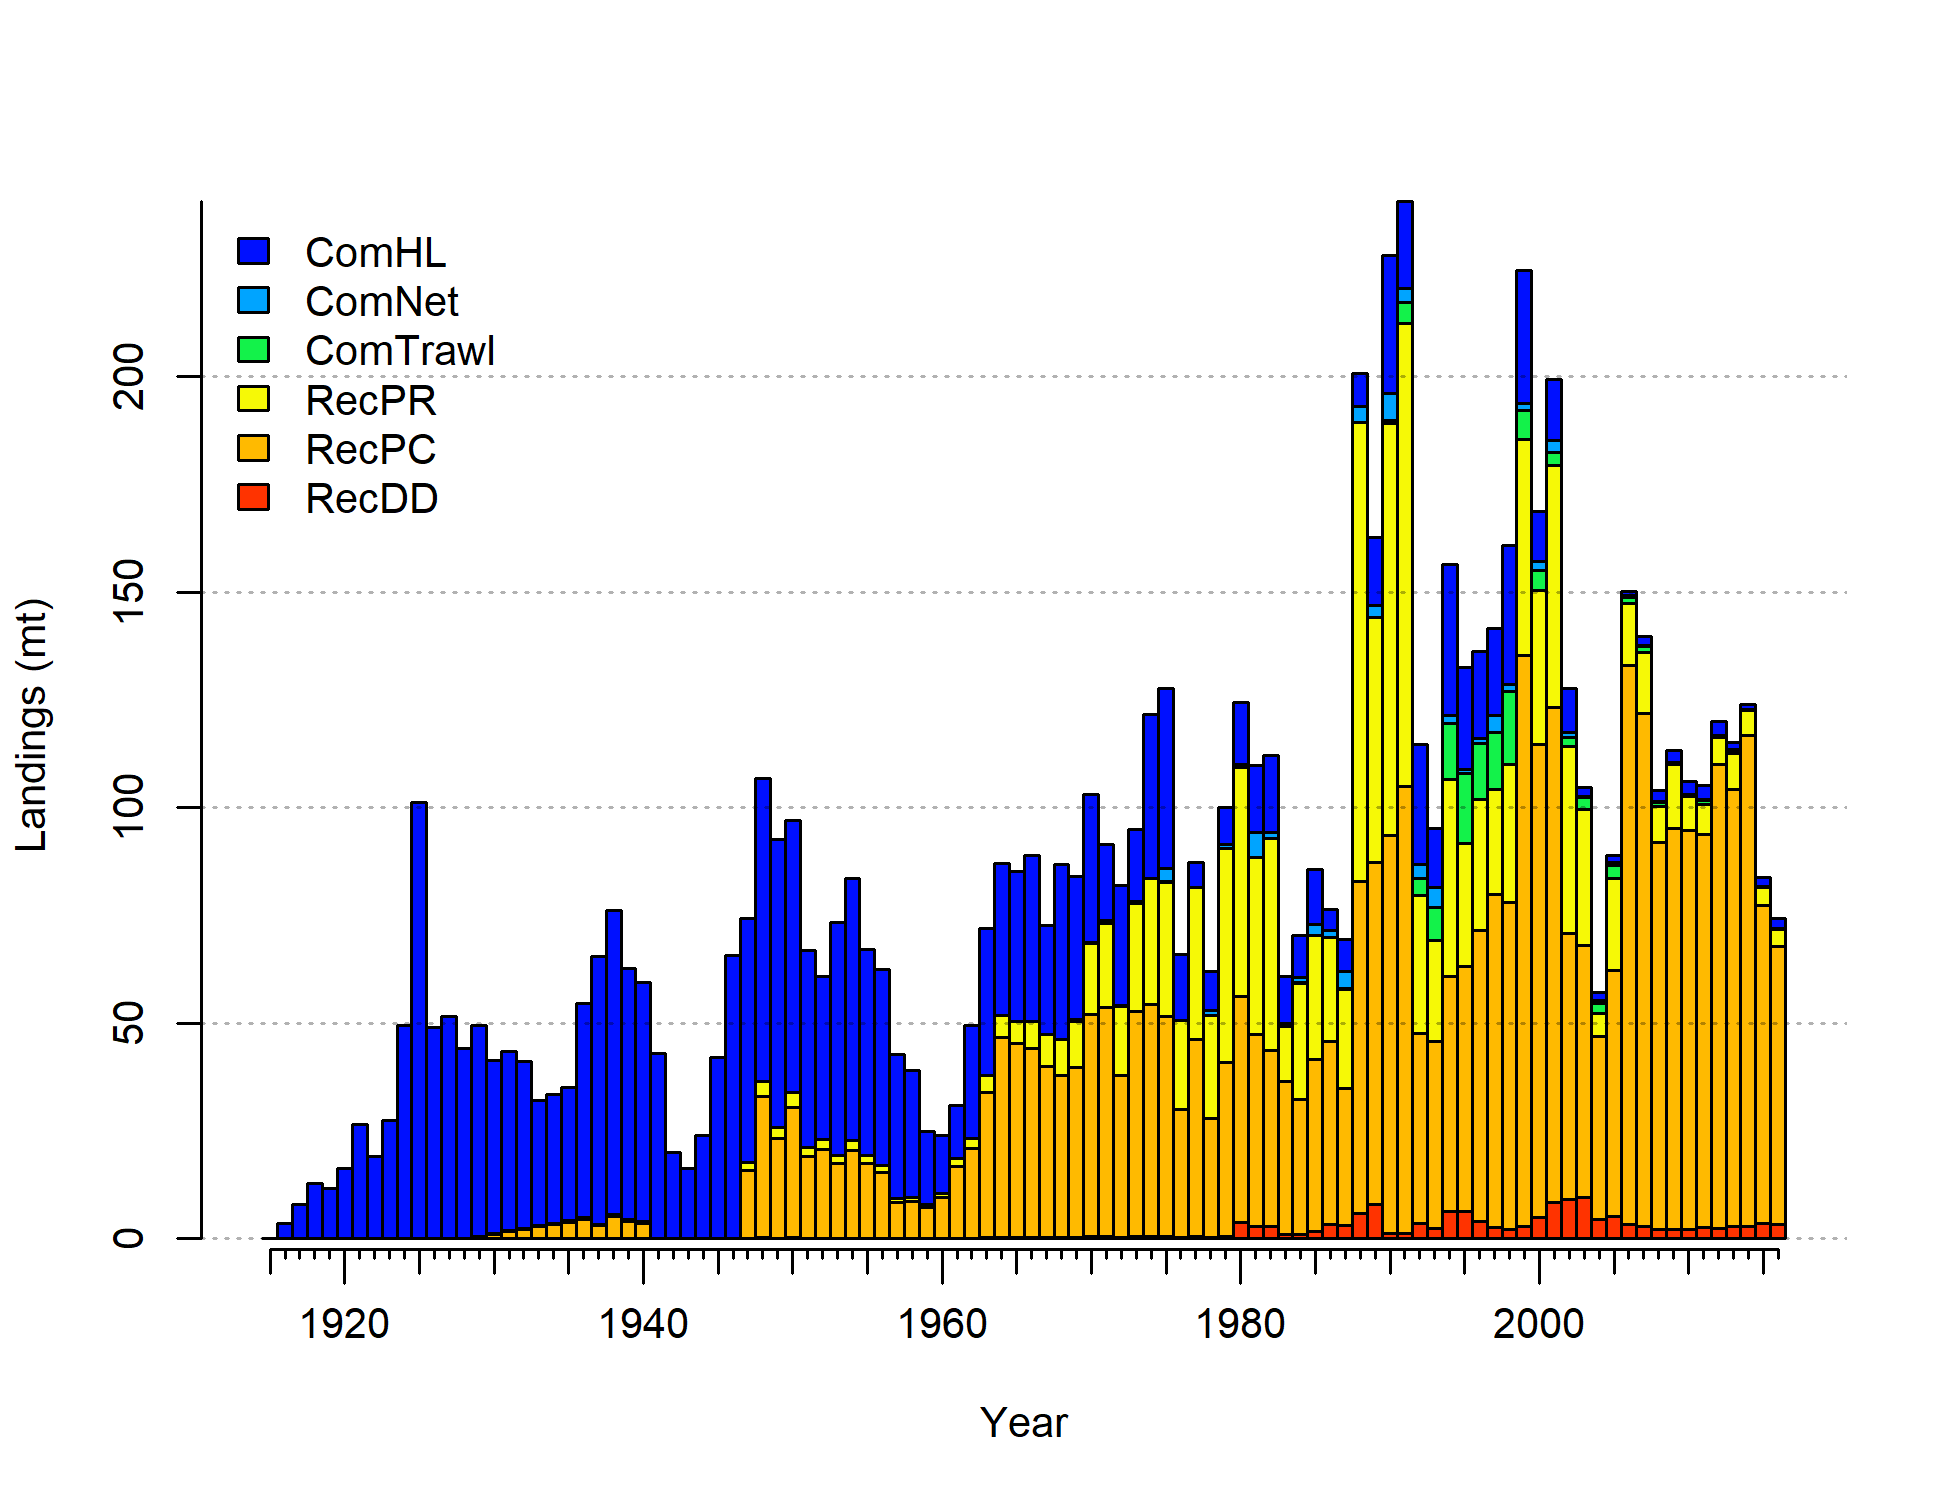
\includegraphics{r4ss/plots_mod1/catch2 landings stacked.png}

\end{frame}

\begin{frame}{Indices of Abundance}

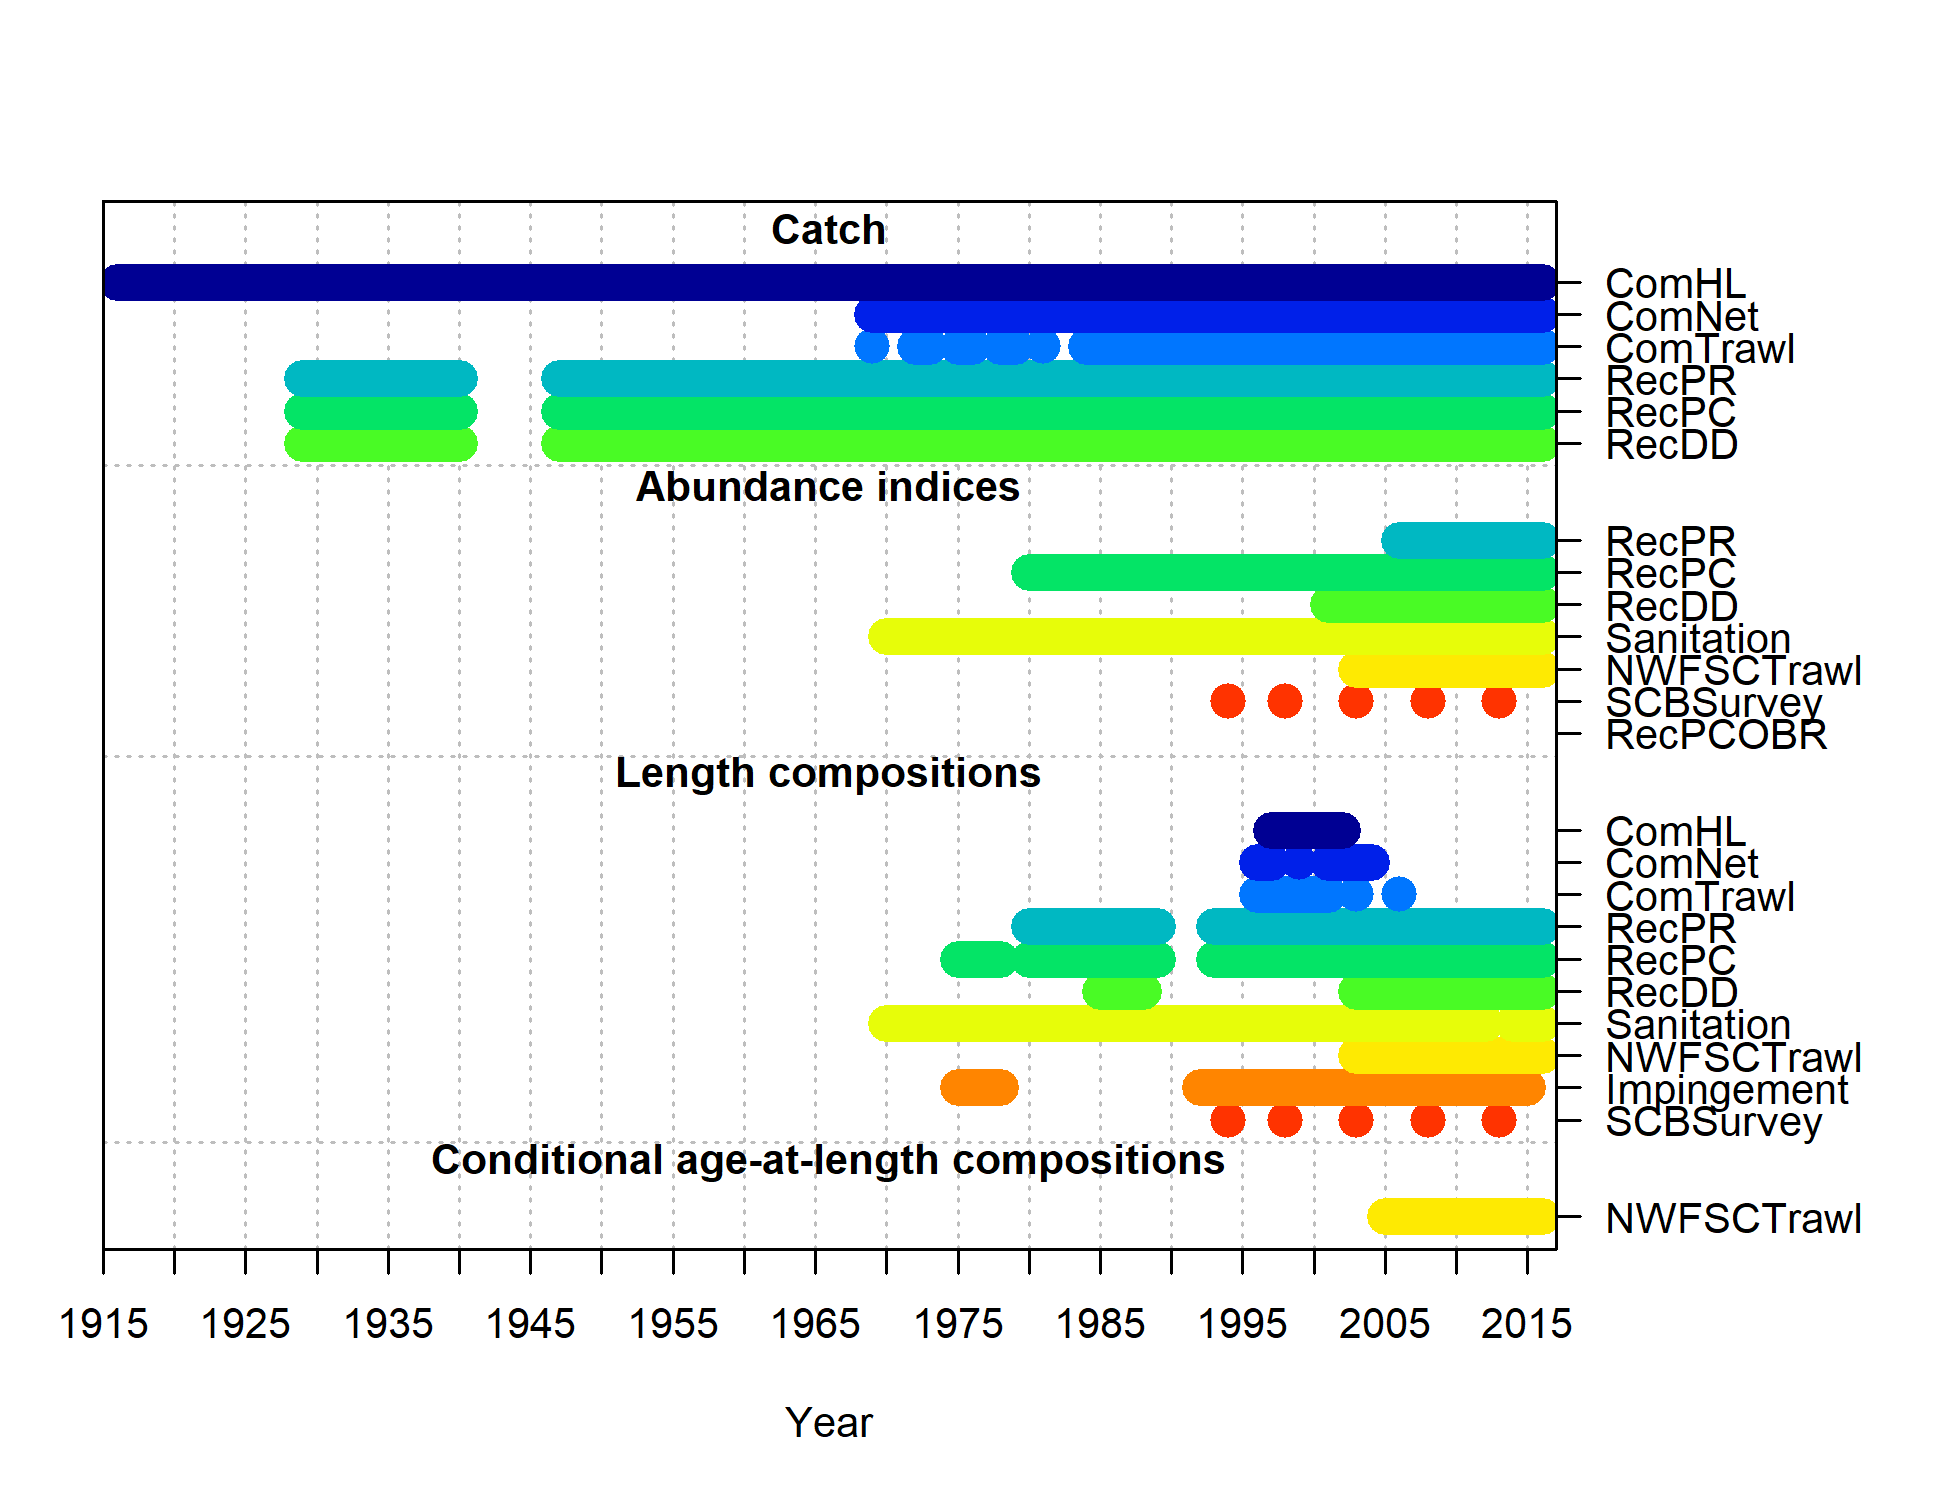
\includegraphics{r4ss/plots_mod1/data_plot.png}

\end{frame}

\begin{frame}{Indices of Abundance}

\begin{itemize}
\tightlist
\item
  All of the methods used to standardize indices have been endorsed by
  the SSC
\end{itemize}

\begin{table}[ht]
\centering
\scalebox{0.7}{
\begin{tabular}{p{2.5in}p{0.8in}p{.4in}p{2in}}
  \hline
Name & Years & Fishery ind. & Method \\ 
  \hline
Recreational PR dockside CPUE & 2004-2016 & No & delta-GLM (bin-lognormal) \\ 
  CPFV logbook CPUE & 1980-2016 & No & negative binomial \\ 
  Onboard observer discard catch CPUE & 2002-2016 & No & delta-GLM (bin-lognormal) \\ 
  Sanitation district CPUE & 1970-2016 & Yes & delta-GLM (bin-lognormal) \\ 
  NWFSC trawl survey CPUE & 2003-2016 & Yes & VAST \\ 
  CSUN/VRG Gillnet survey CPUE & 1995-2008 & Yes & delta-GLM (bin-lognormal) \\ 
  Southern California Bight trawl survey CPUE & '94, '98, '03, '08, '13 & Yes & delta-GLM (bin-lognormal) \\ 
  Onboard observer retained catch CPUE & 2002-2016 & No & delta-GLM (bin-lognormal) \\ 
   \hline
\end{tabular}
}
\end{table}

\end{frame}

\begin{frame}{Indices of Abundance}

\begincols
 \begincol{.5\textwidth}

\begin{itemize}
\item[$\bullet$] Stephens-MacCall threshold exploration for the dockside recreational charter boat index
\item[$\bullet$] Index not used in the assessment, charter boat logbook used
\end{itemize}

\endcol
 \begincol{.5\textwidth}
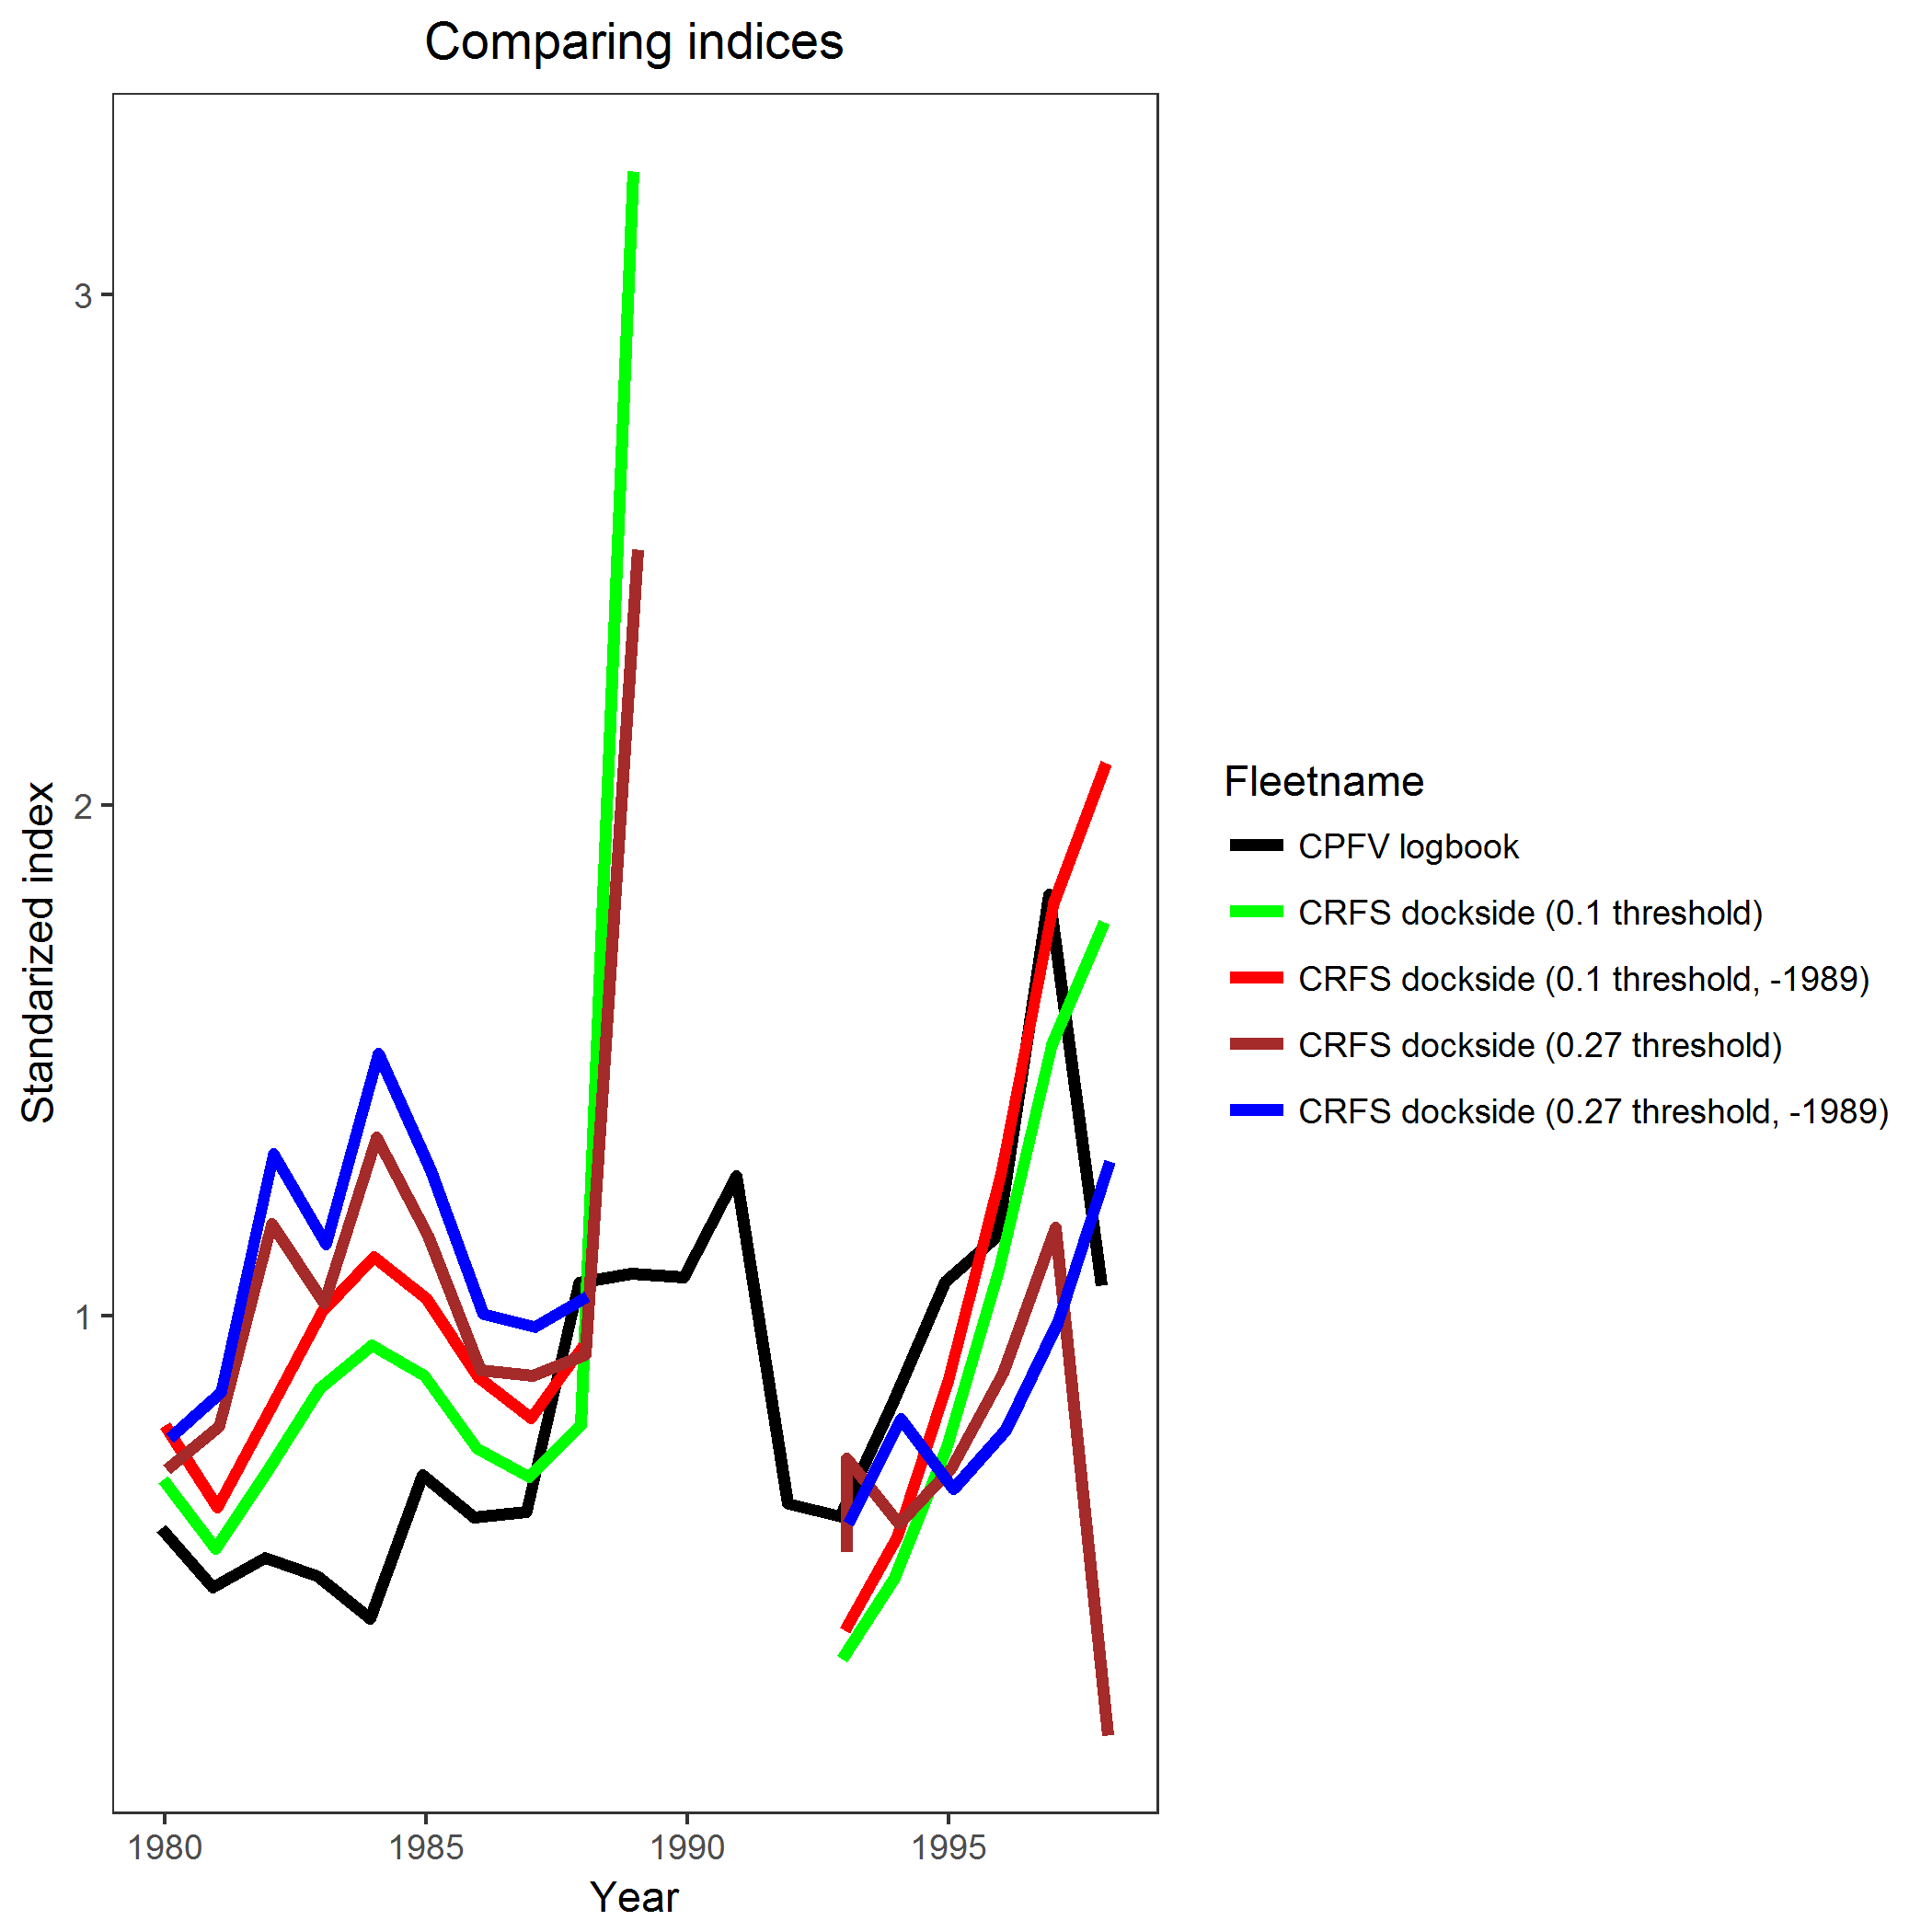
\includegraphics{Figures/Fleet5_RecPC_dockside_index_compare.png}
\endcol
\endcols

\end{frame}

\begin{frame}{All Indices of Abundance}

The gillnet survey removed from the final model
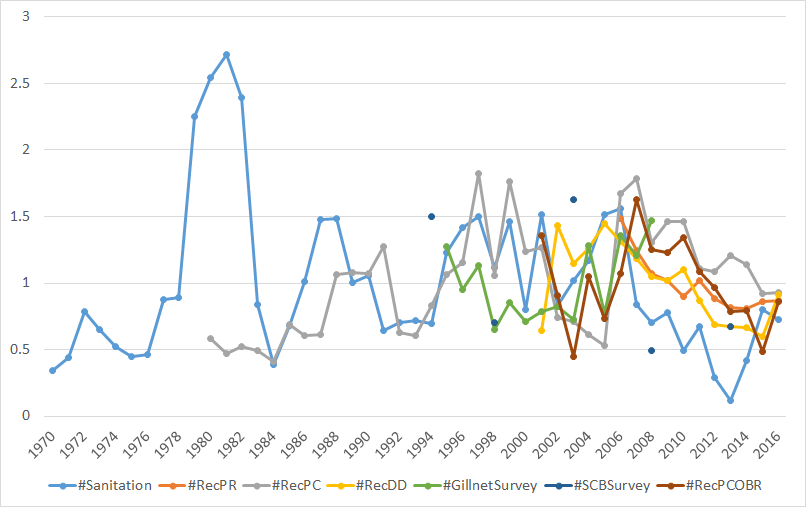
\includegraphics{Figures/All_indices.png}

\end{frame}

\begin{frame}{Aggregate length composition}

\centering

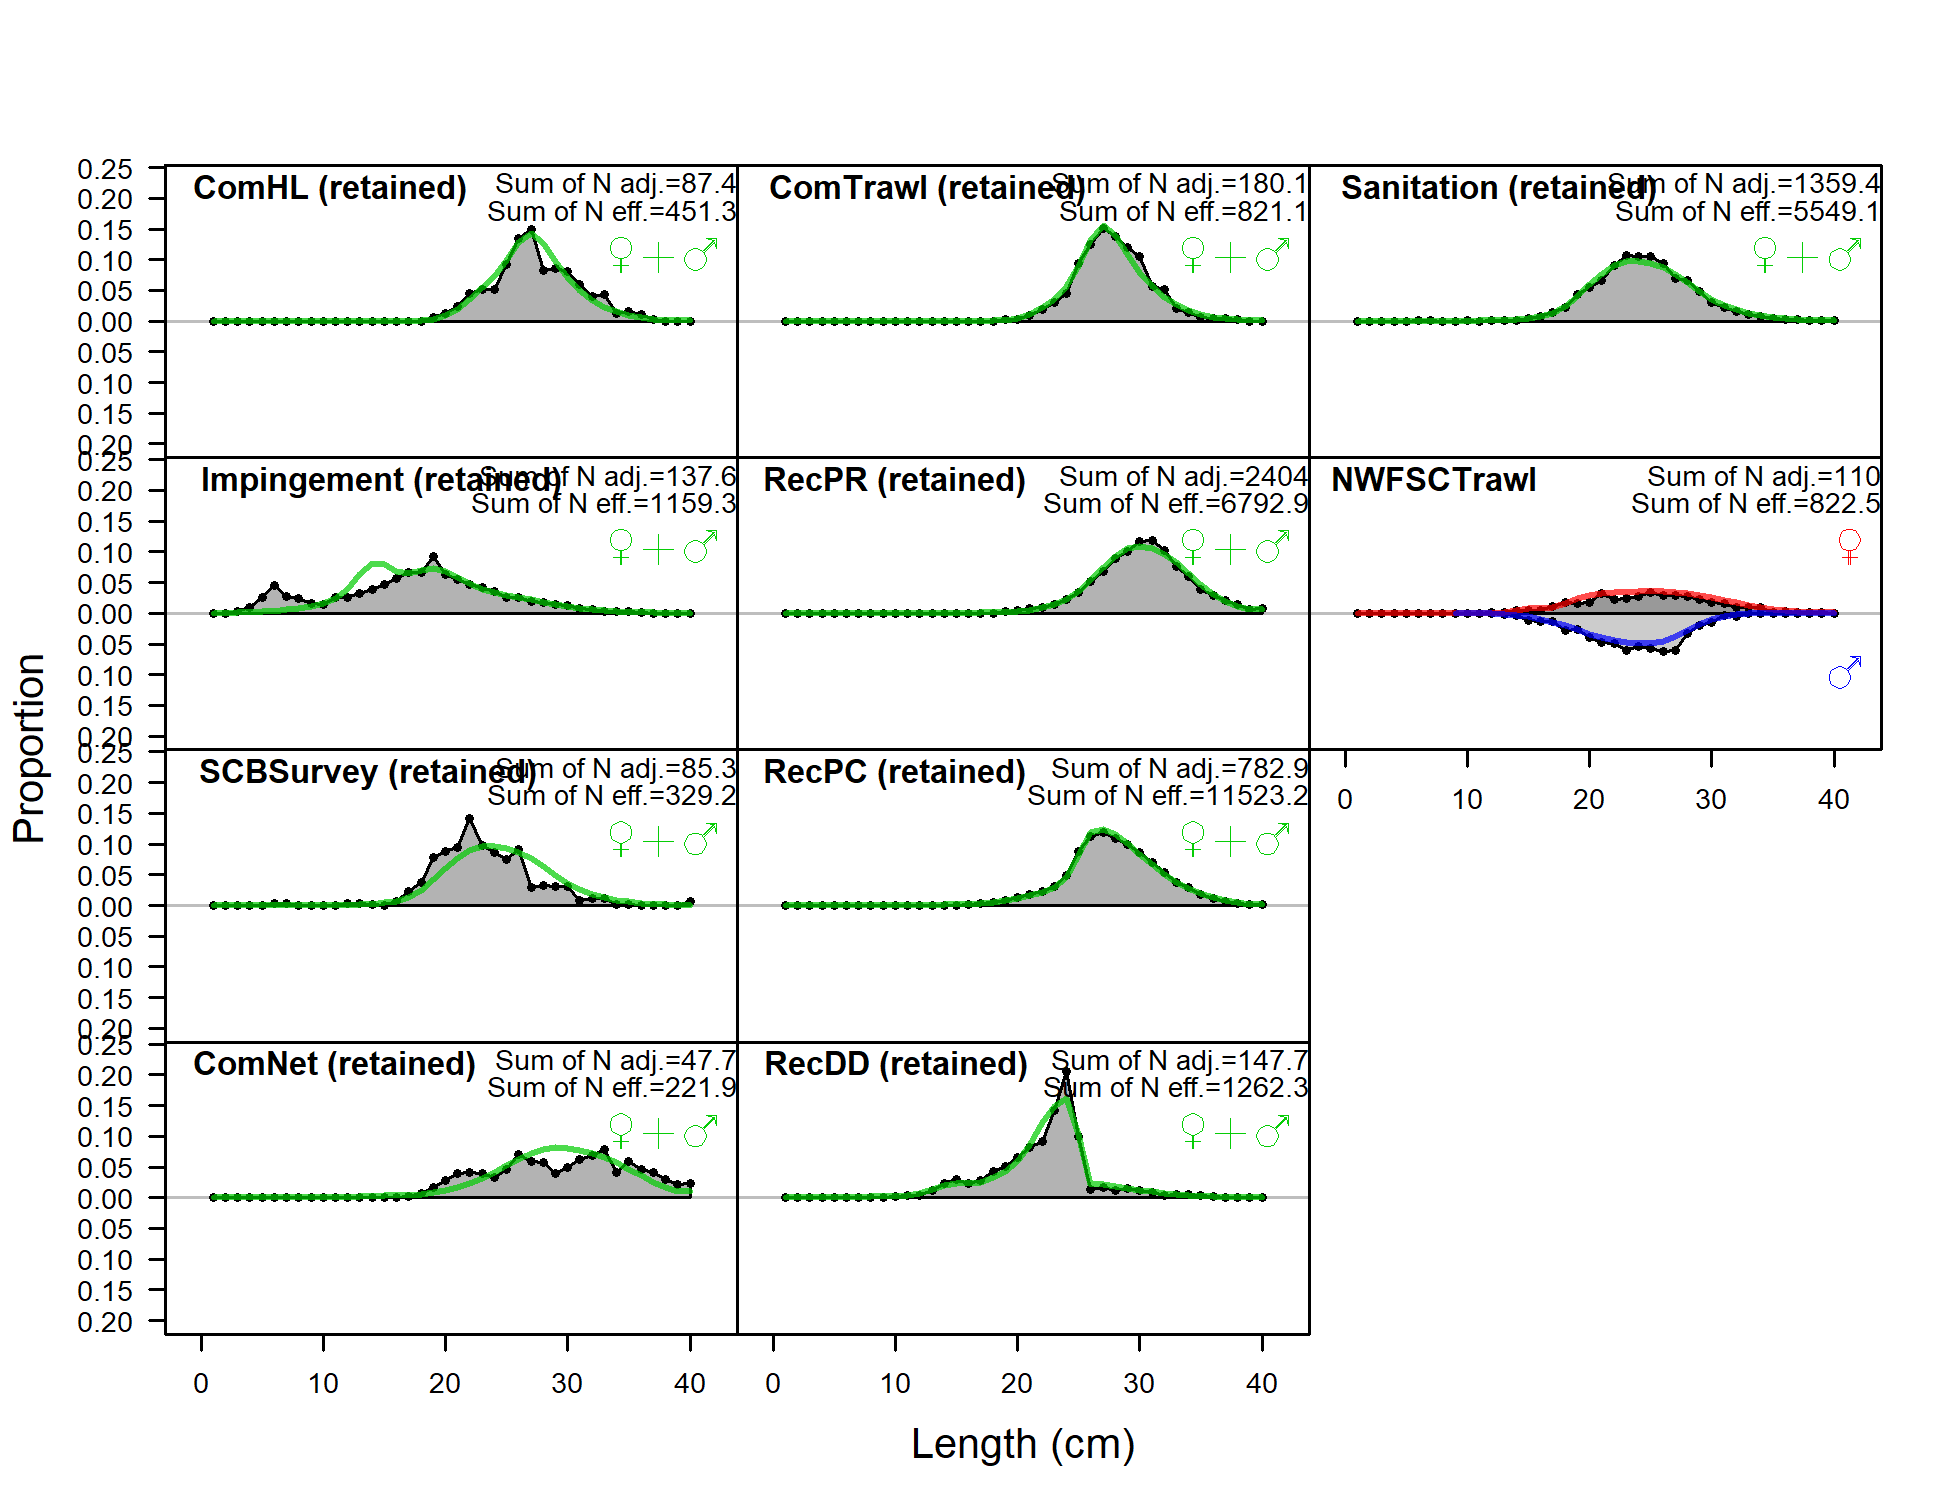
\includegraphics{r4ss/plots_mod1/comp_lenfit__aggregated_across_time.png}

\end{frame}

\begin{frame}{NWFSC Length and Age Composition}

Note: females in red and males in blue \begincols
 \begincol{.5\textwidth}
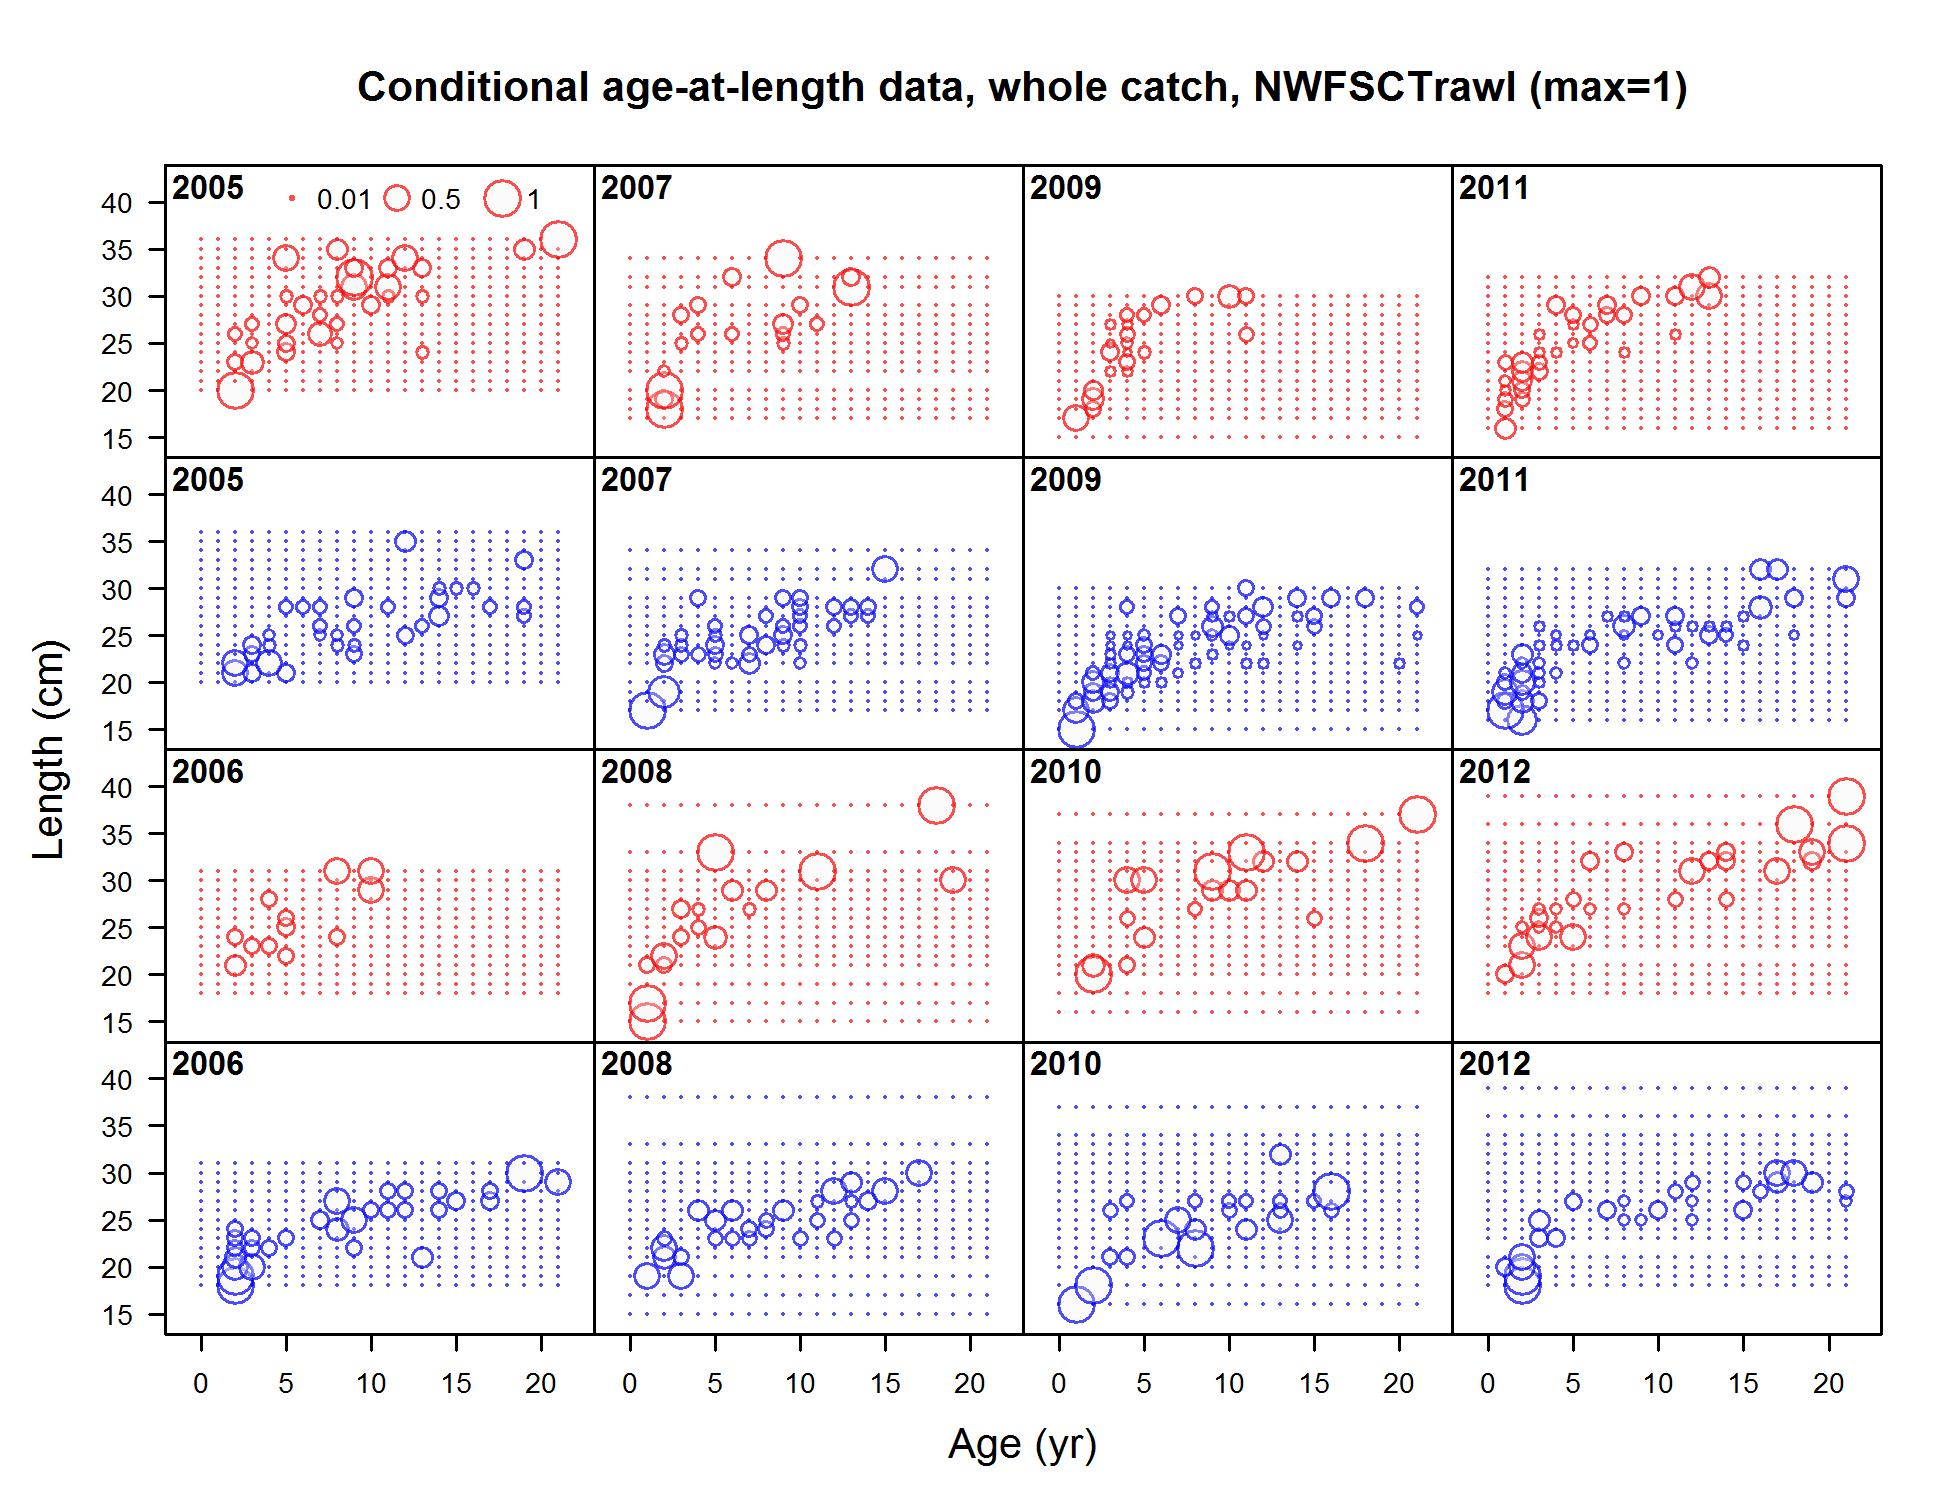
\includegraphics[height=.5\textheight]{r4ss/plots_mod1/comp_condAALdat_bubflt8mkt0_page1.png}
\endcol
 \begincol{.5\textwidth}
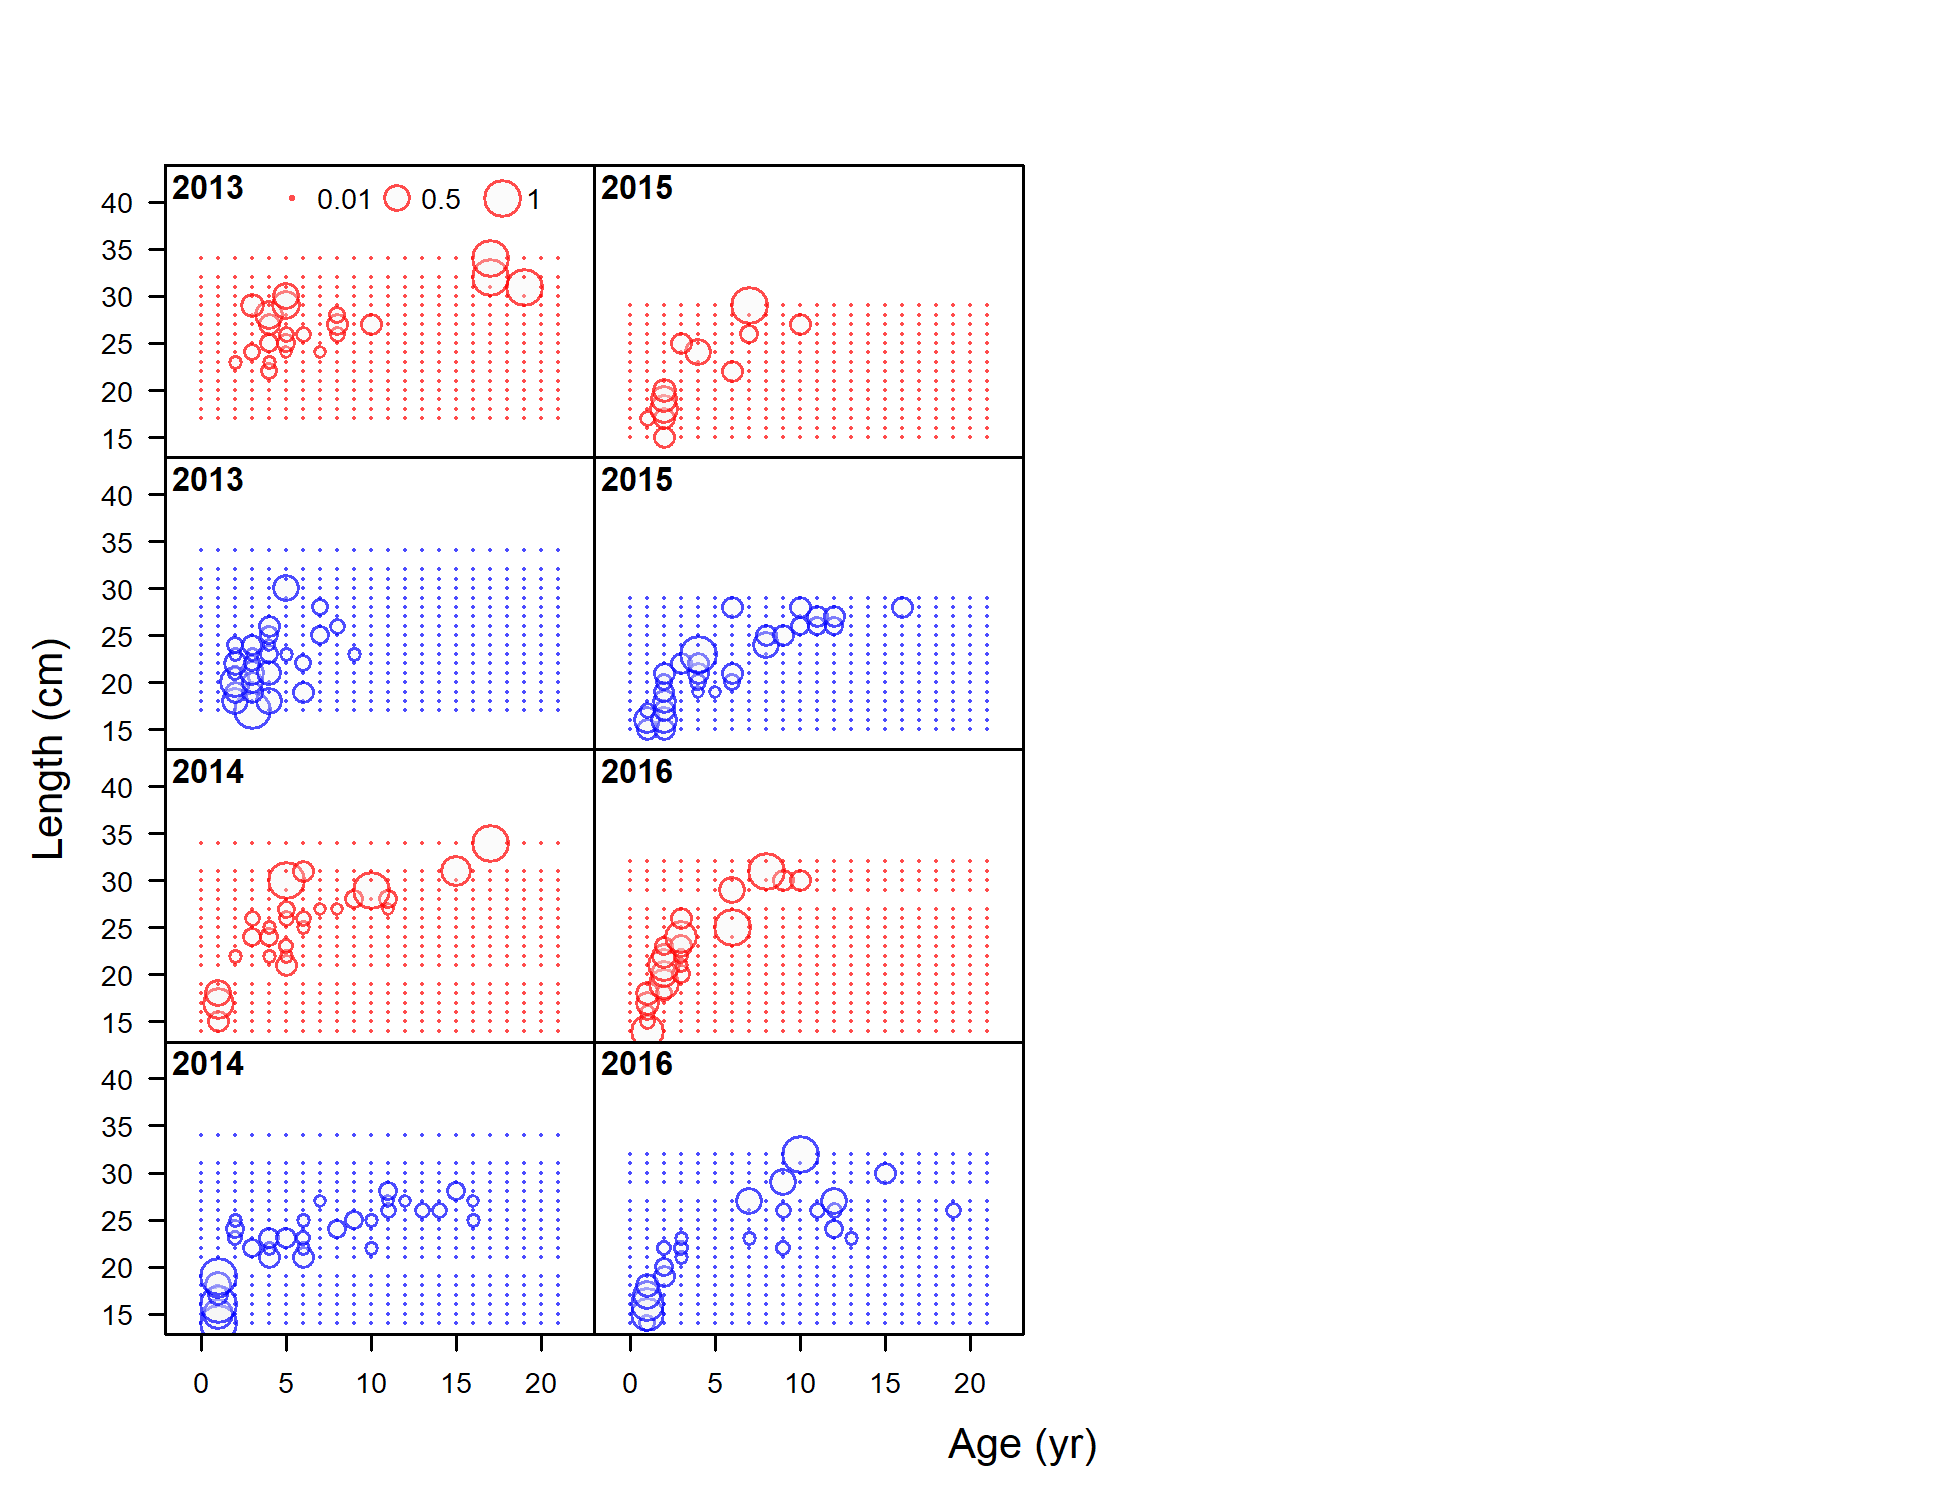
\includegraphics[height=.5\textheight]{r4ss/plots_mod1/comp_condAALdat_bubflt8mkt0_page2.png}
\endcol
\endcols

\end{frame}

\begin{frame}{Length-at-Age}

\begincols
 \begincol{.4\textwidth}
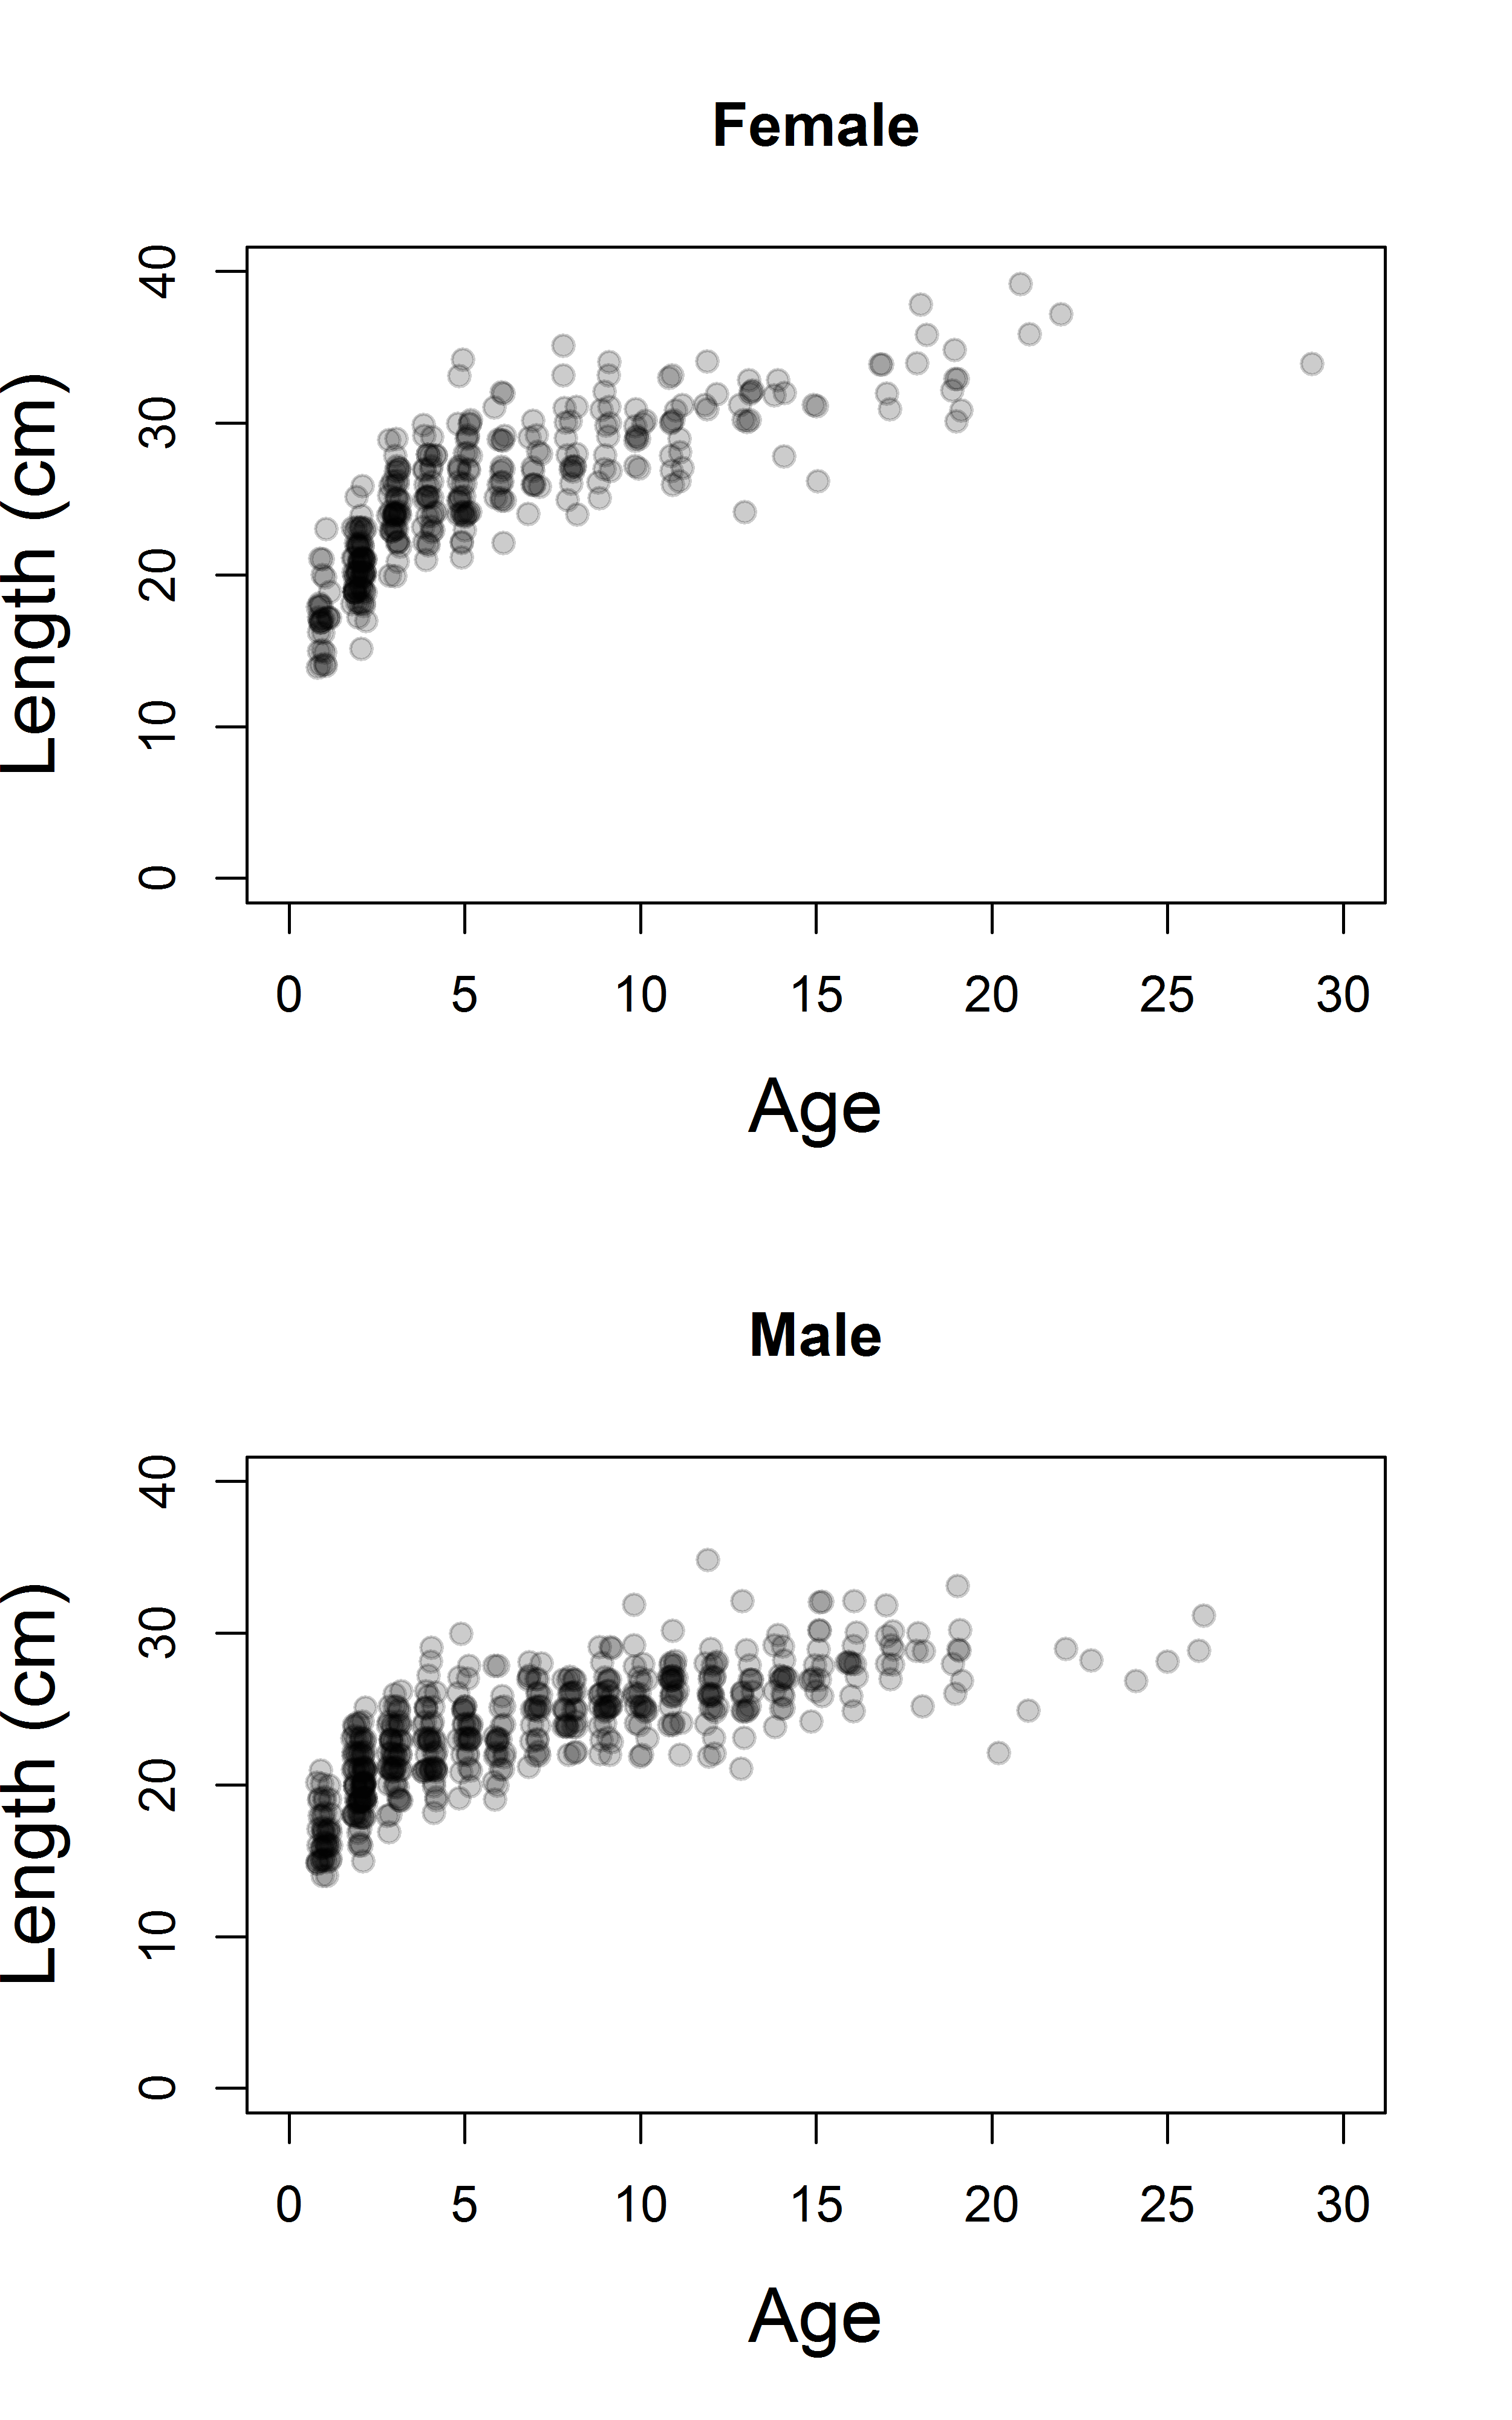
\includegraphics[trim={0 0 0 2cm}, totalheight=0.65\textheight]{Figures/Age_length_bySex.png}
\endcol
 \begincol{.48\textwidth} 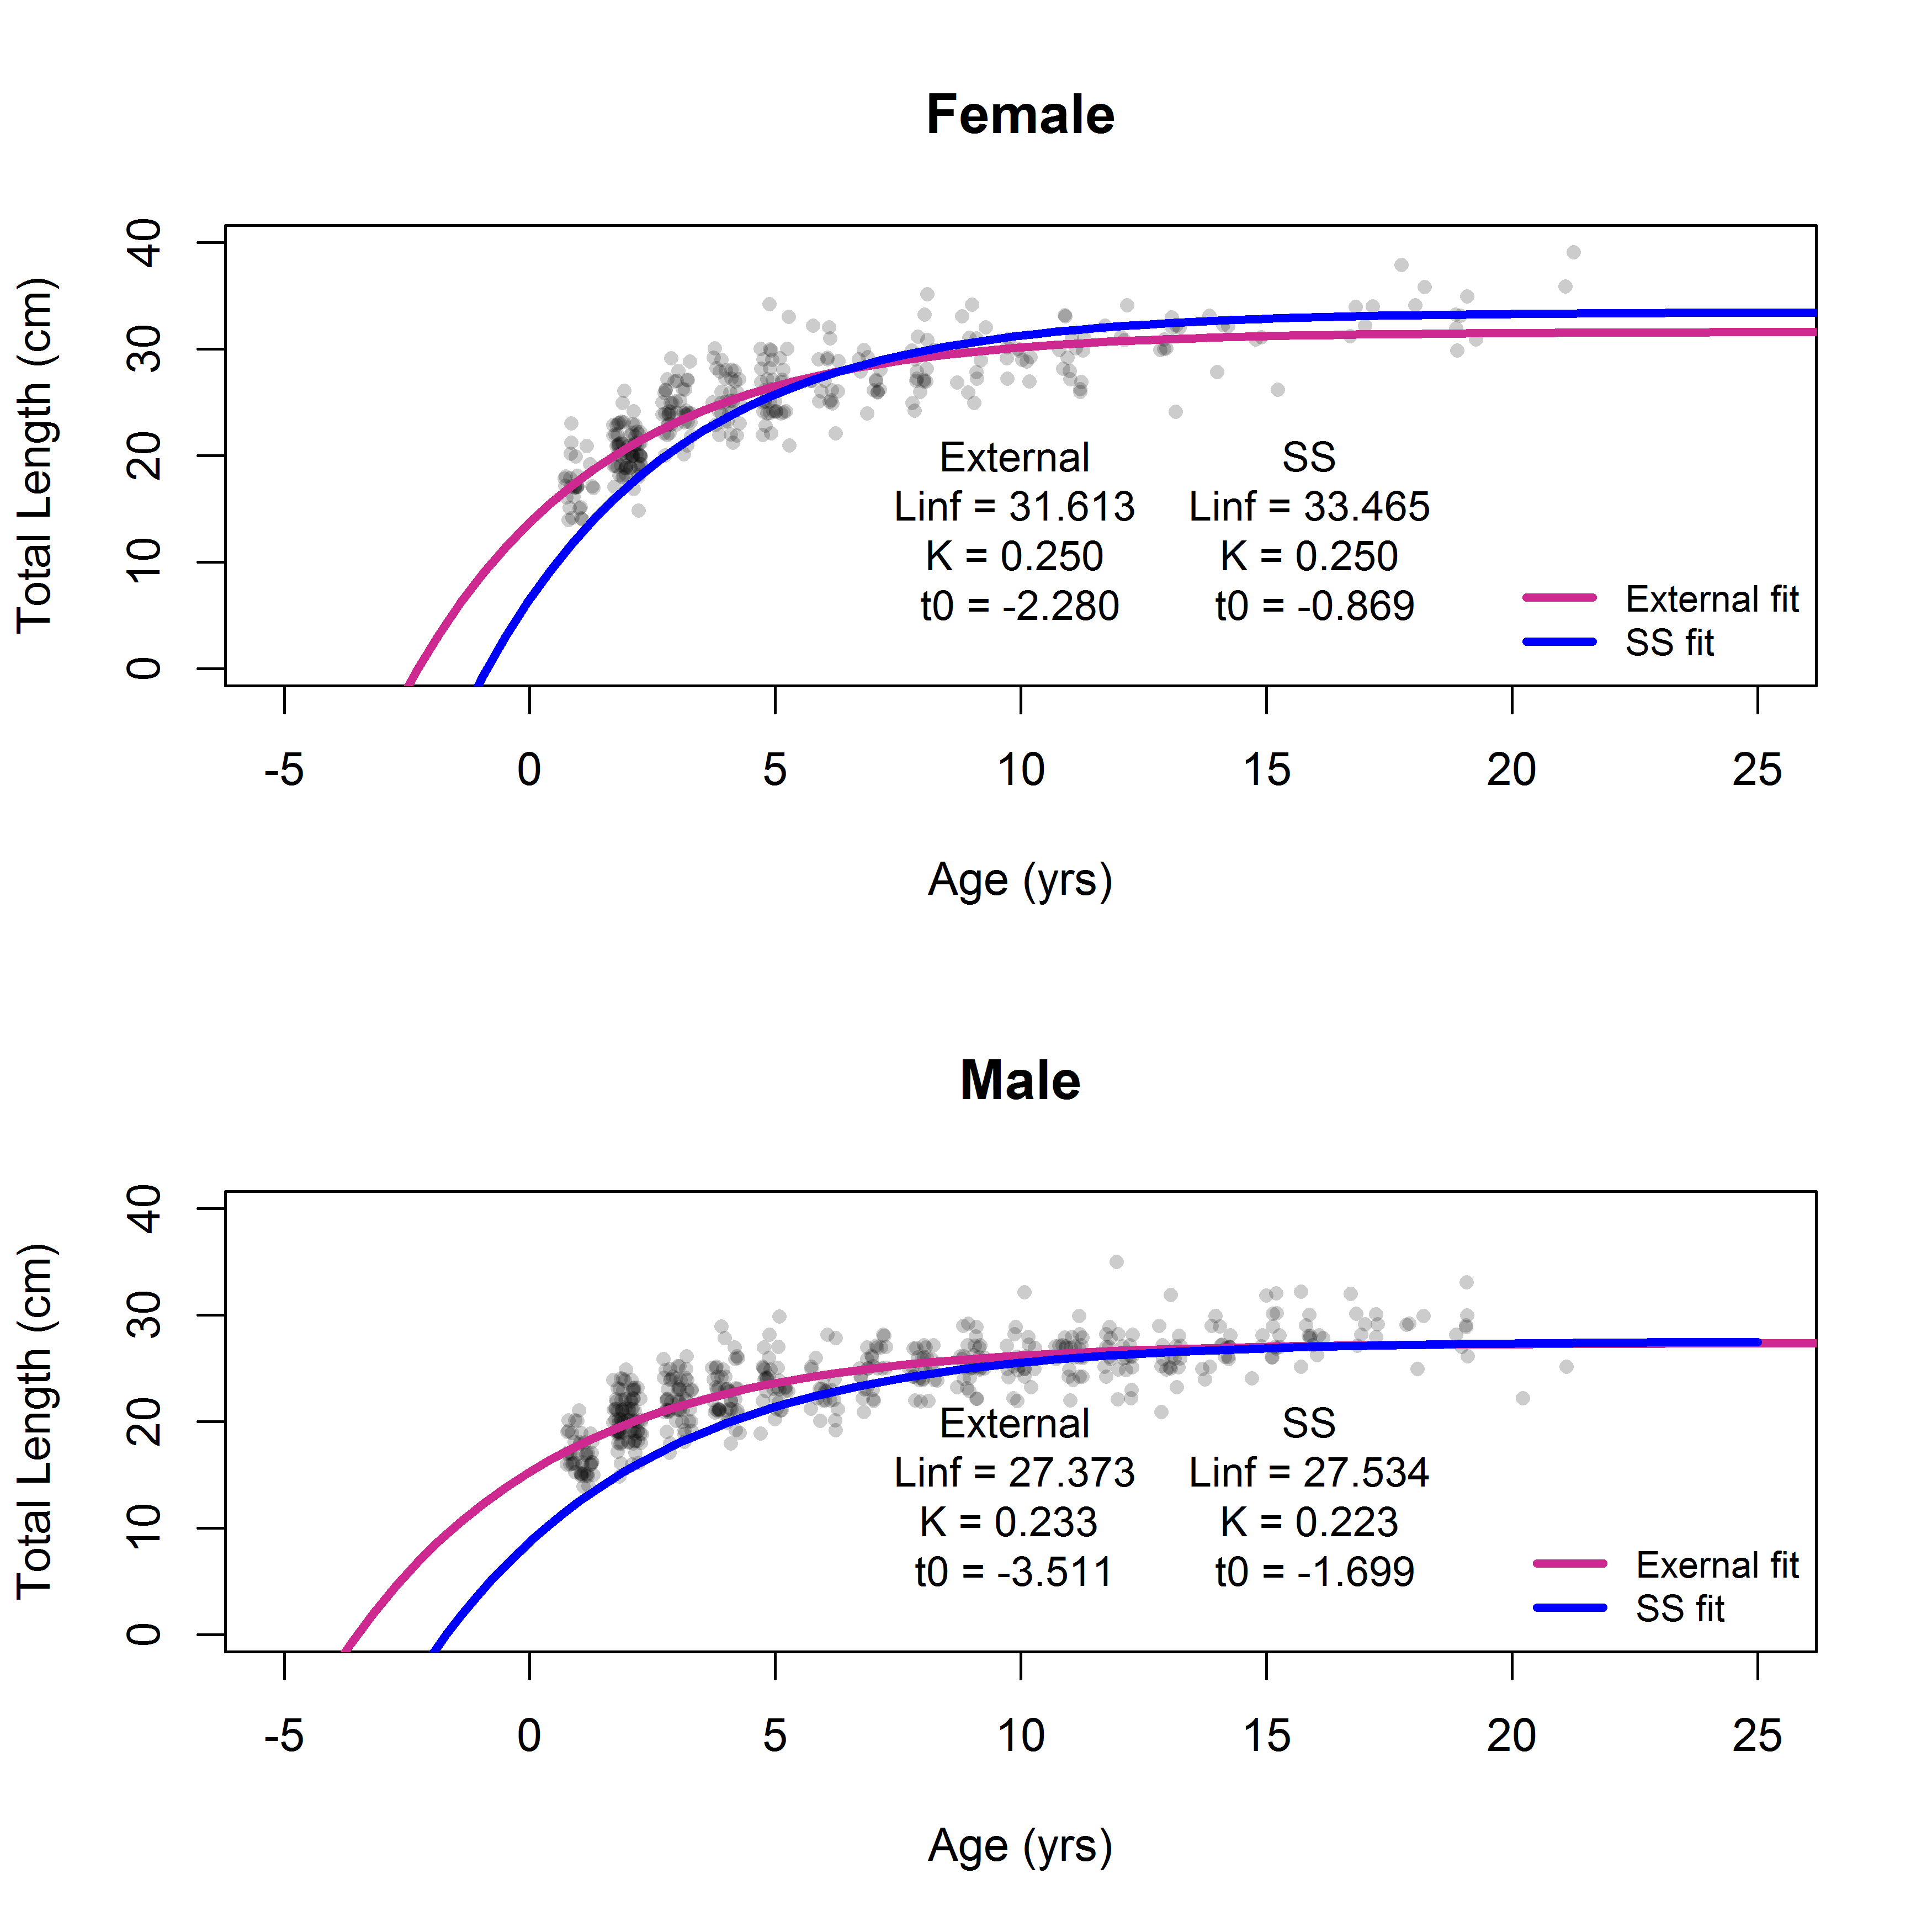
\includegraphics{Figures/vonB_compare.png}
\endcol
\endcols

\end{frame}

\begin{frame}{Model Specifications}

\begin{itemize}
\item[$\bullet$] Stock Synthesis version 3.30.05.04
\item[$\bullet$] Model starts in 1916, unfished equilibrium catch prior to that
\item[$\bullet$] $M$ fixed at 0.235 for both sexes
\begin{itemize}
\item[$\circ$] Pre-STAR model fixed female $M$ at prior with max. age of 21 (0.25714), male $M$ offset estimated
\item[$\circ$] $M$ fixed at 0.25 for both sexes in 2005 assessment
\end{itemize}
\item[$\bullet$] Steepness fixed at 0.718 (from meta-analysis)
\begin{itemize}
\item[$\circ$] $h$ fixed at 0.7 in 2005 assessment
\end{itemize}
\item[$\bullet$] One cm length bins
\item[$\bullet$] Recruitment deviations estimated
\end{itemize}

\end{frame}

\begin{frame}{Selectivity}

\begin{itemize}
\item[$\bullet$] Time blocks
\begin{itemize}
\item[$\circ$] Commercial fleet: 1916-1999 and 2000-2016 (10-in. minimum size limit as of 2000)
\item[$\circ$] Recreational fleets: 1916-2000 (few regulations), 2001-2005 (fishery closures), 2006-2016 (consistent regulations)
\end{itemize}
\item[$\bullet$] Double normal selectivity patterns
\end{itemize}

\end{frame}

\begin{frame}{Stock Status - Biomass}

\centering
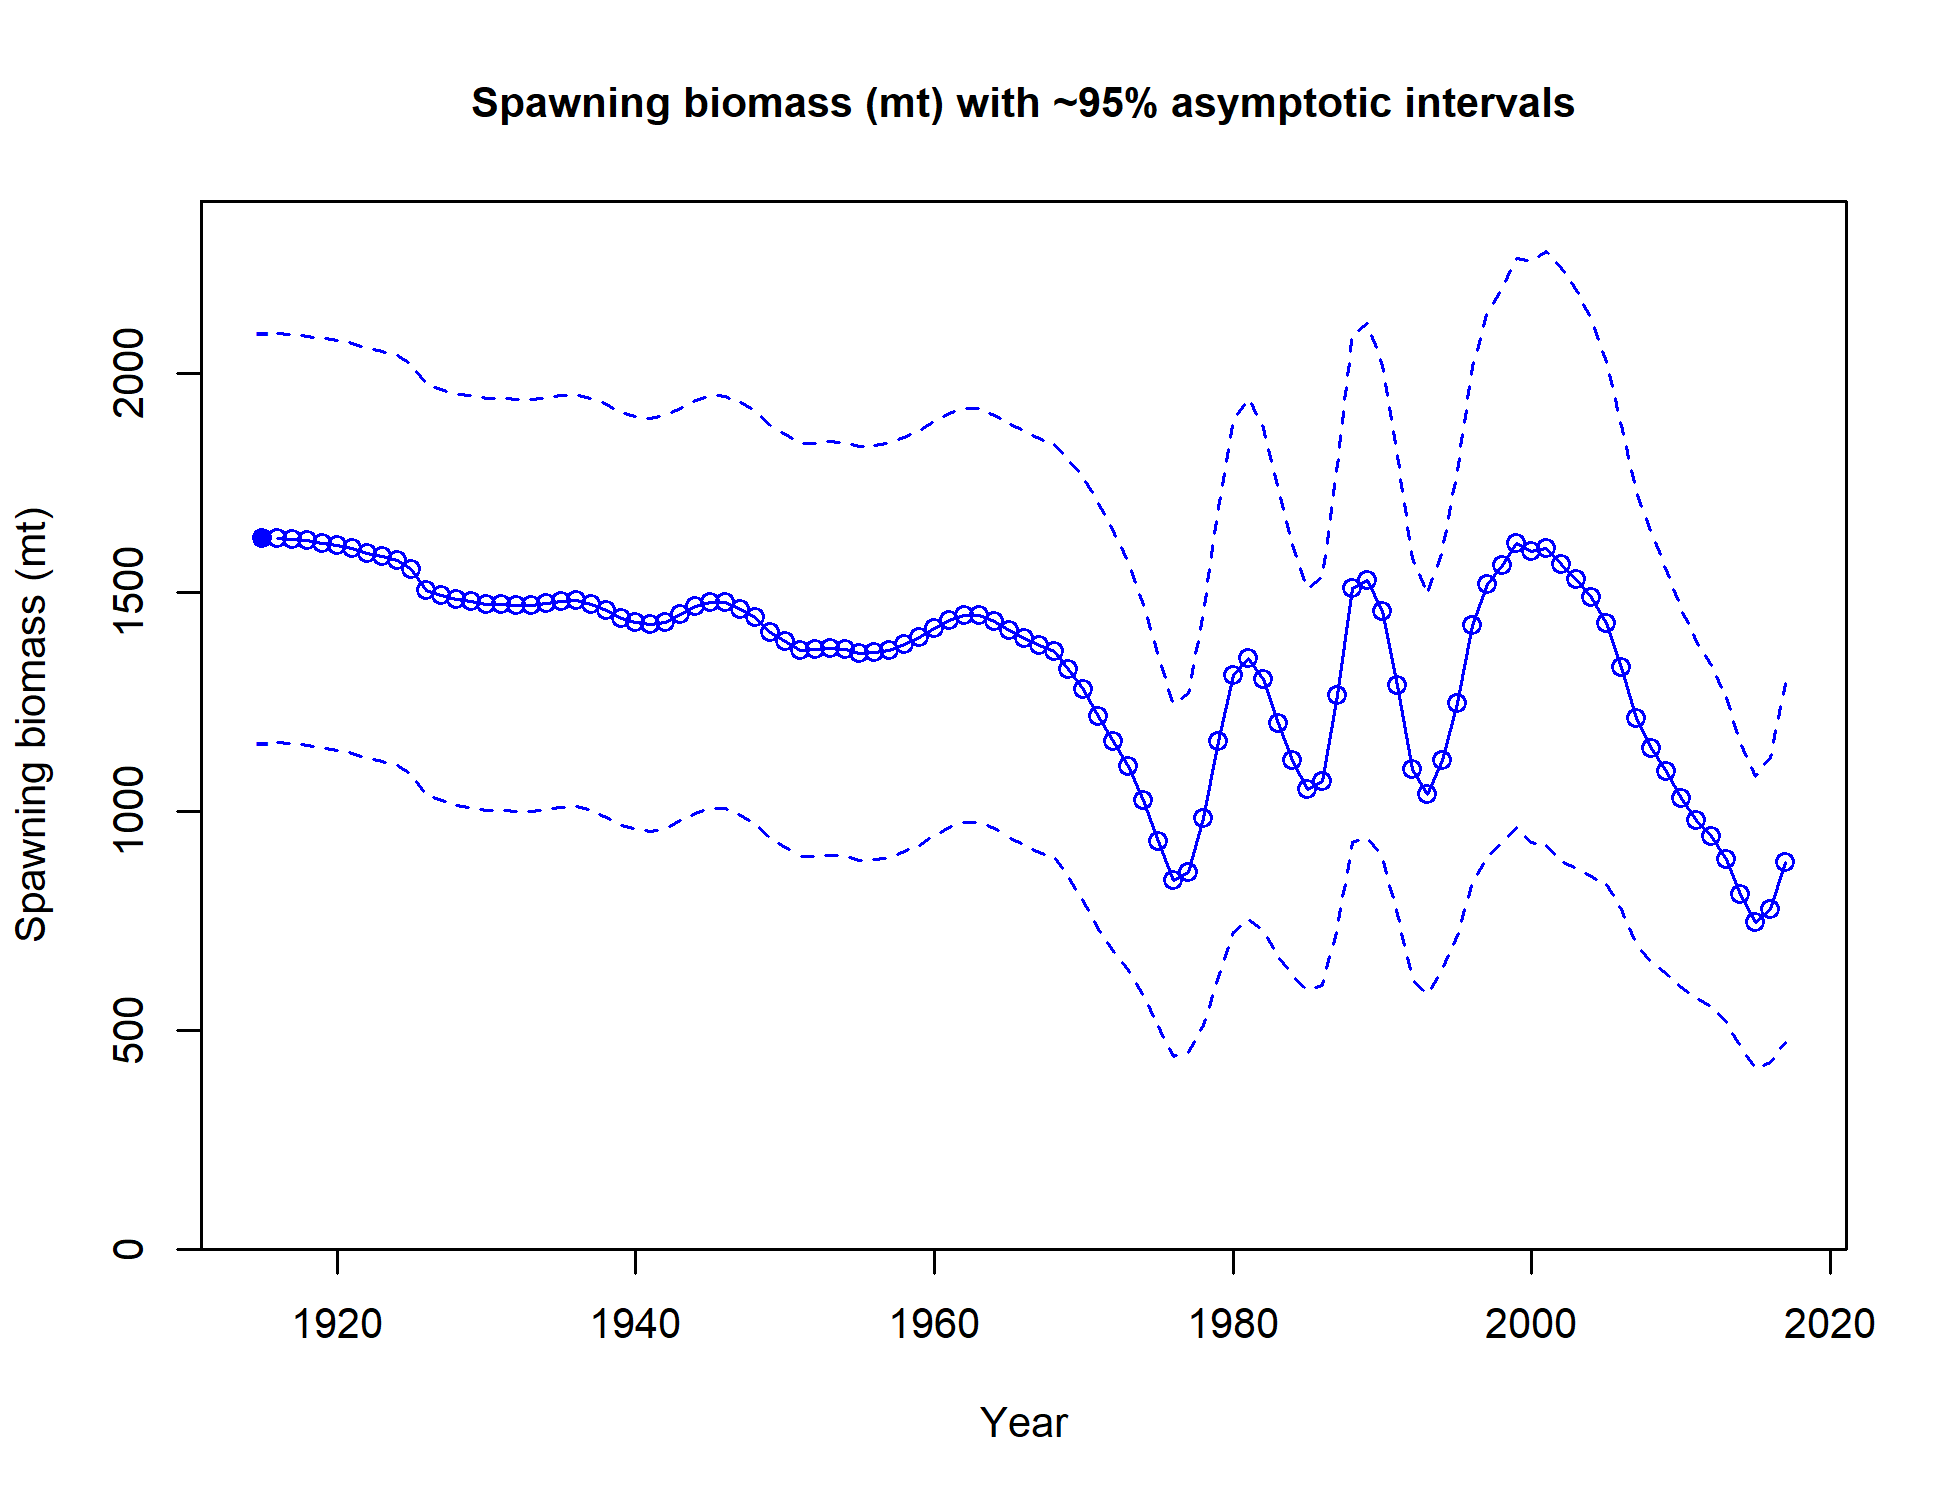
\includegraphics{r4ss/plots_mod1/ts7_Spawning_biomass_(mt)_with_95_asymptotic_intervals_intervals.png}

\end{frame}

\begin{frame}{Stock Status - Depletion}

\centering
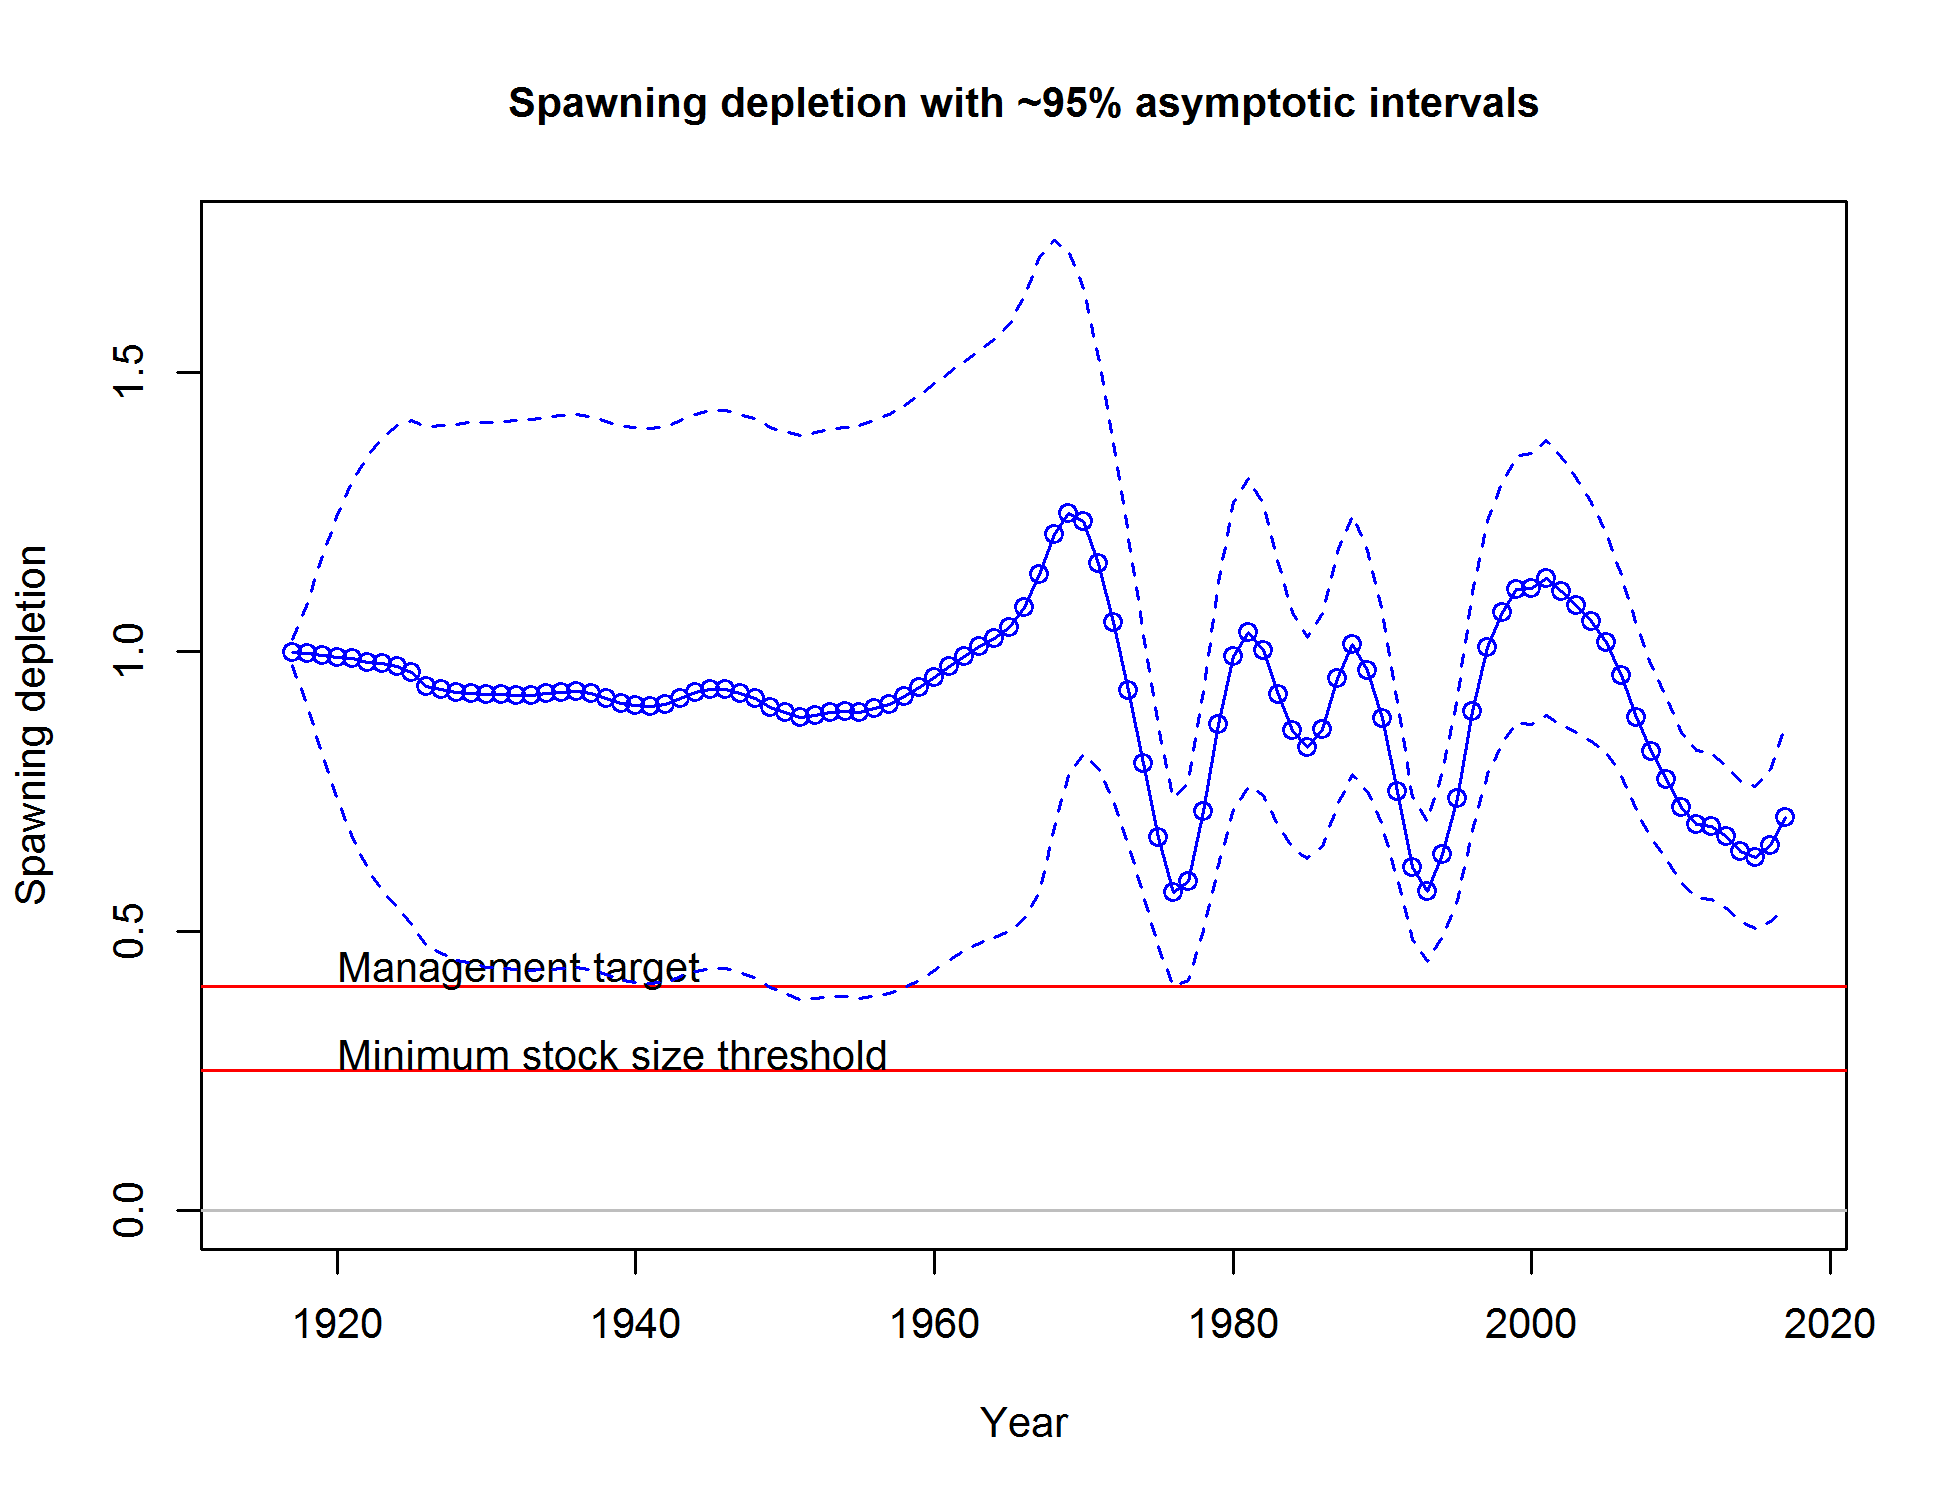
\includegraphics{r4ss/plots_mod1/ts9_Spawning_depletion_with_95_asymptotic_intervals_intervals.png}

\end{frame}

\begin{frame}{Stock Status - Recruitment}

\centering
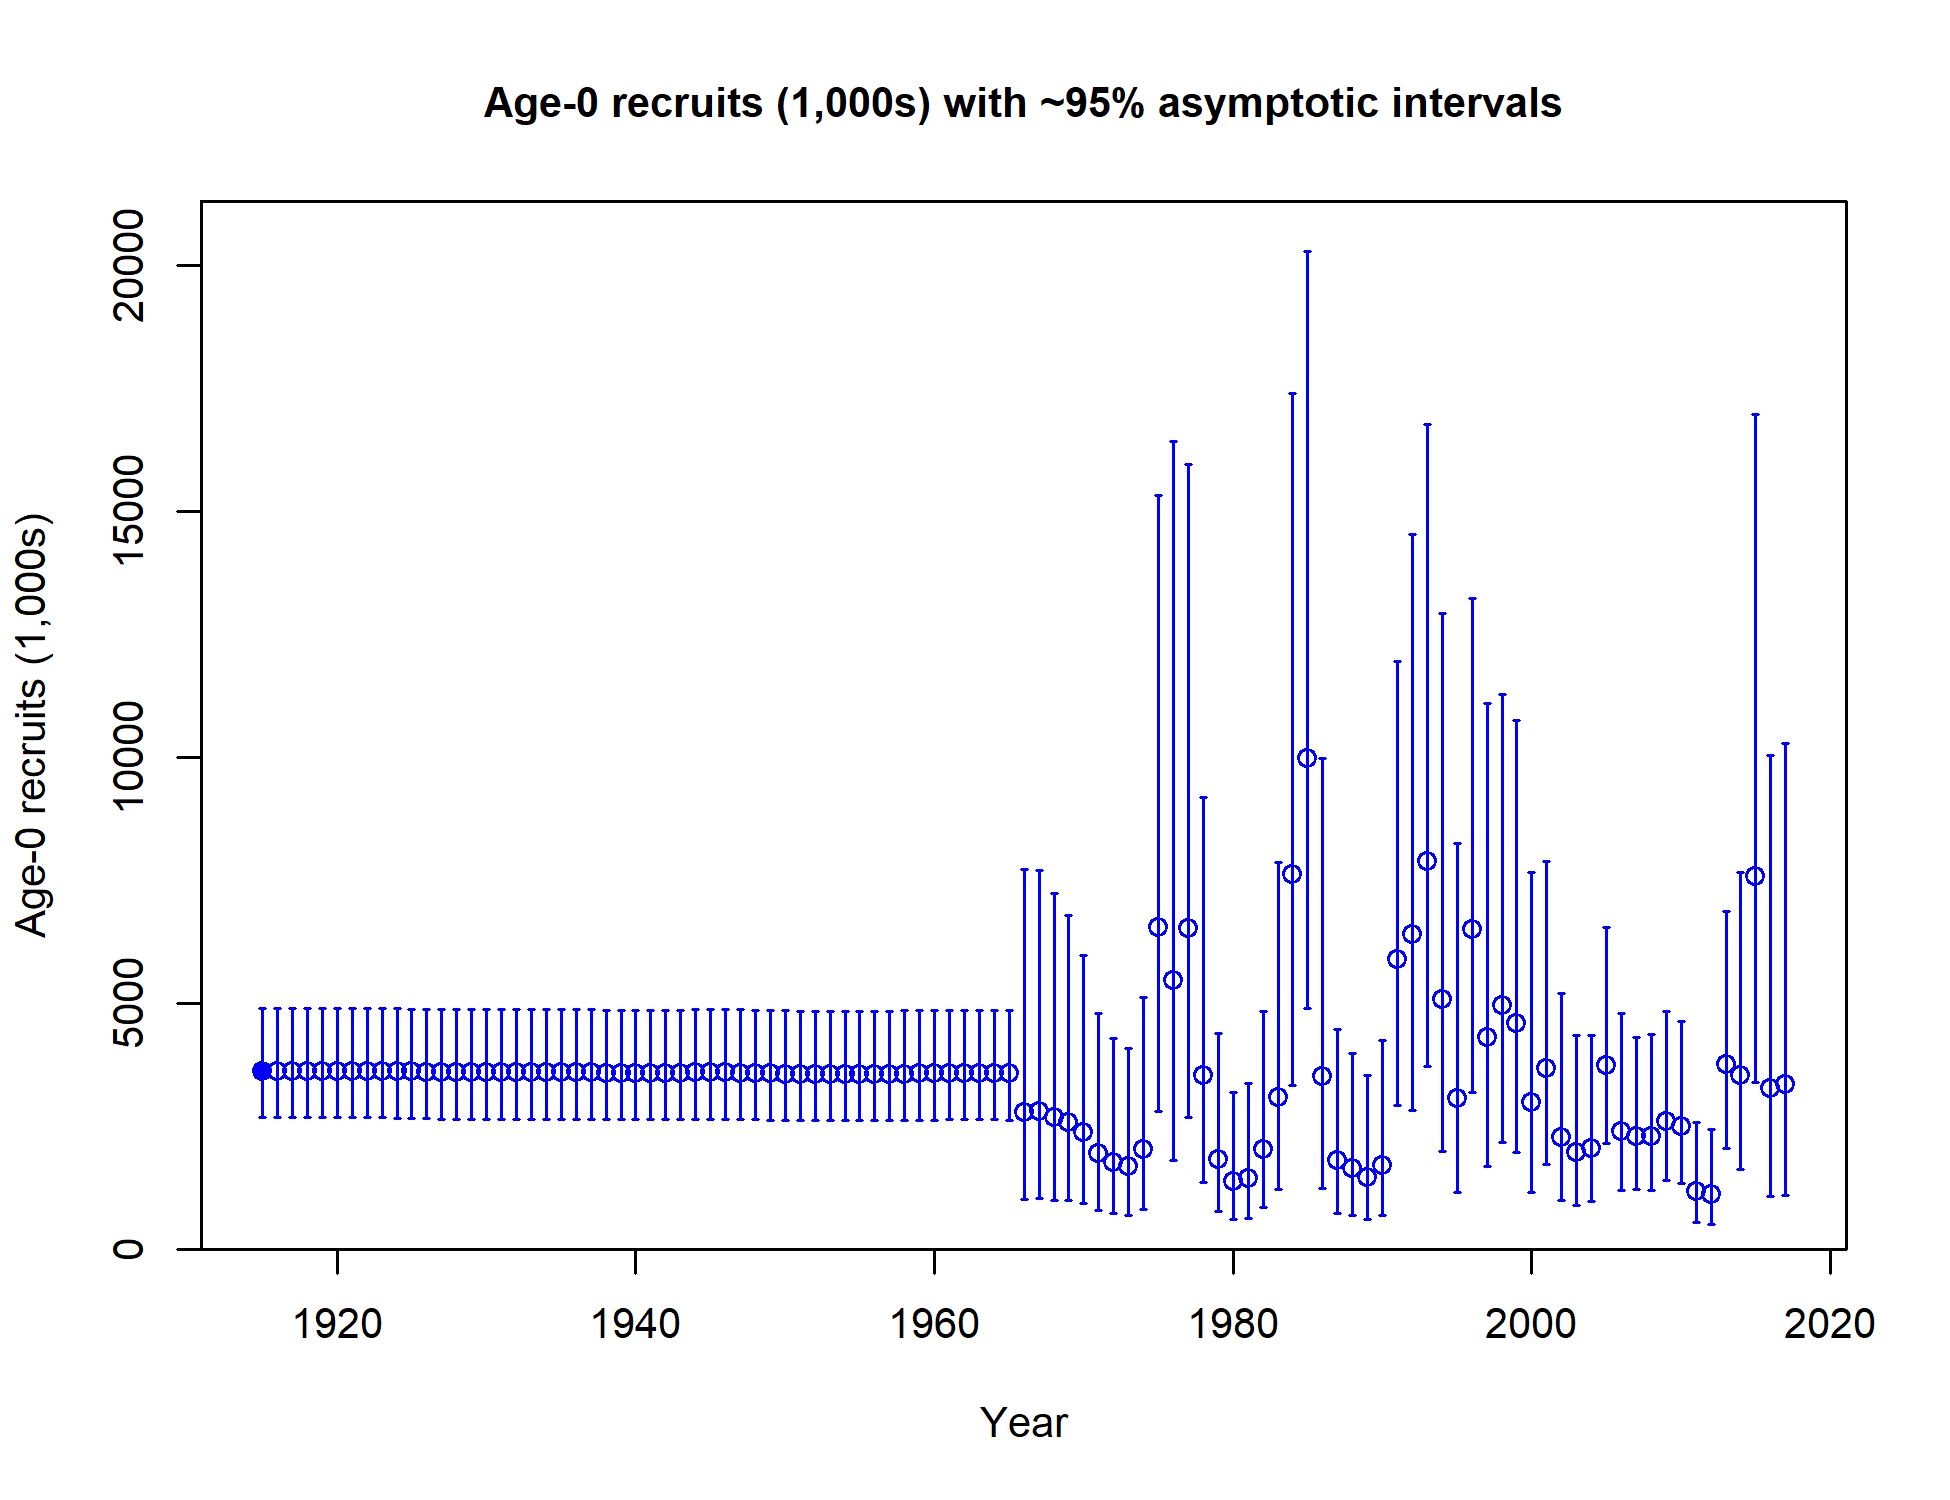
\includegraphics{r4ss/plots_mod1/ts11_Age-0_recruits_(1000s)_with_95_asymptotic_intervals.png}

\end{frame}

\begin{frame}{Stock Status - Exploitation}

\begincols
 \begincol{.5\textwidth}
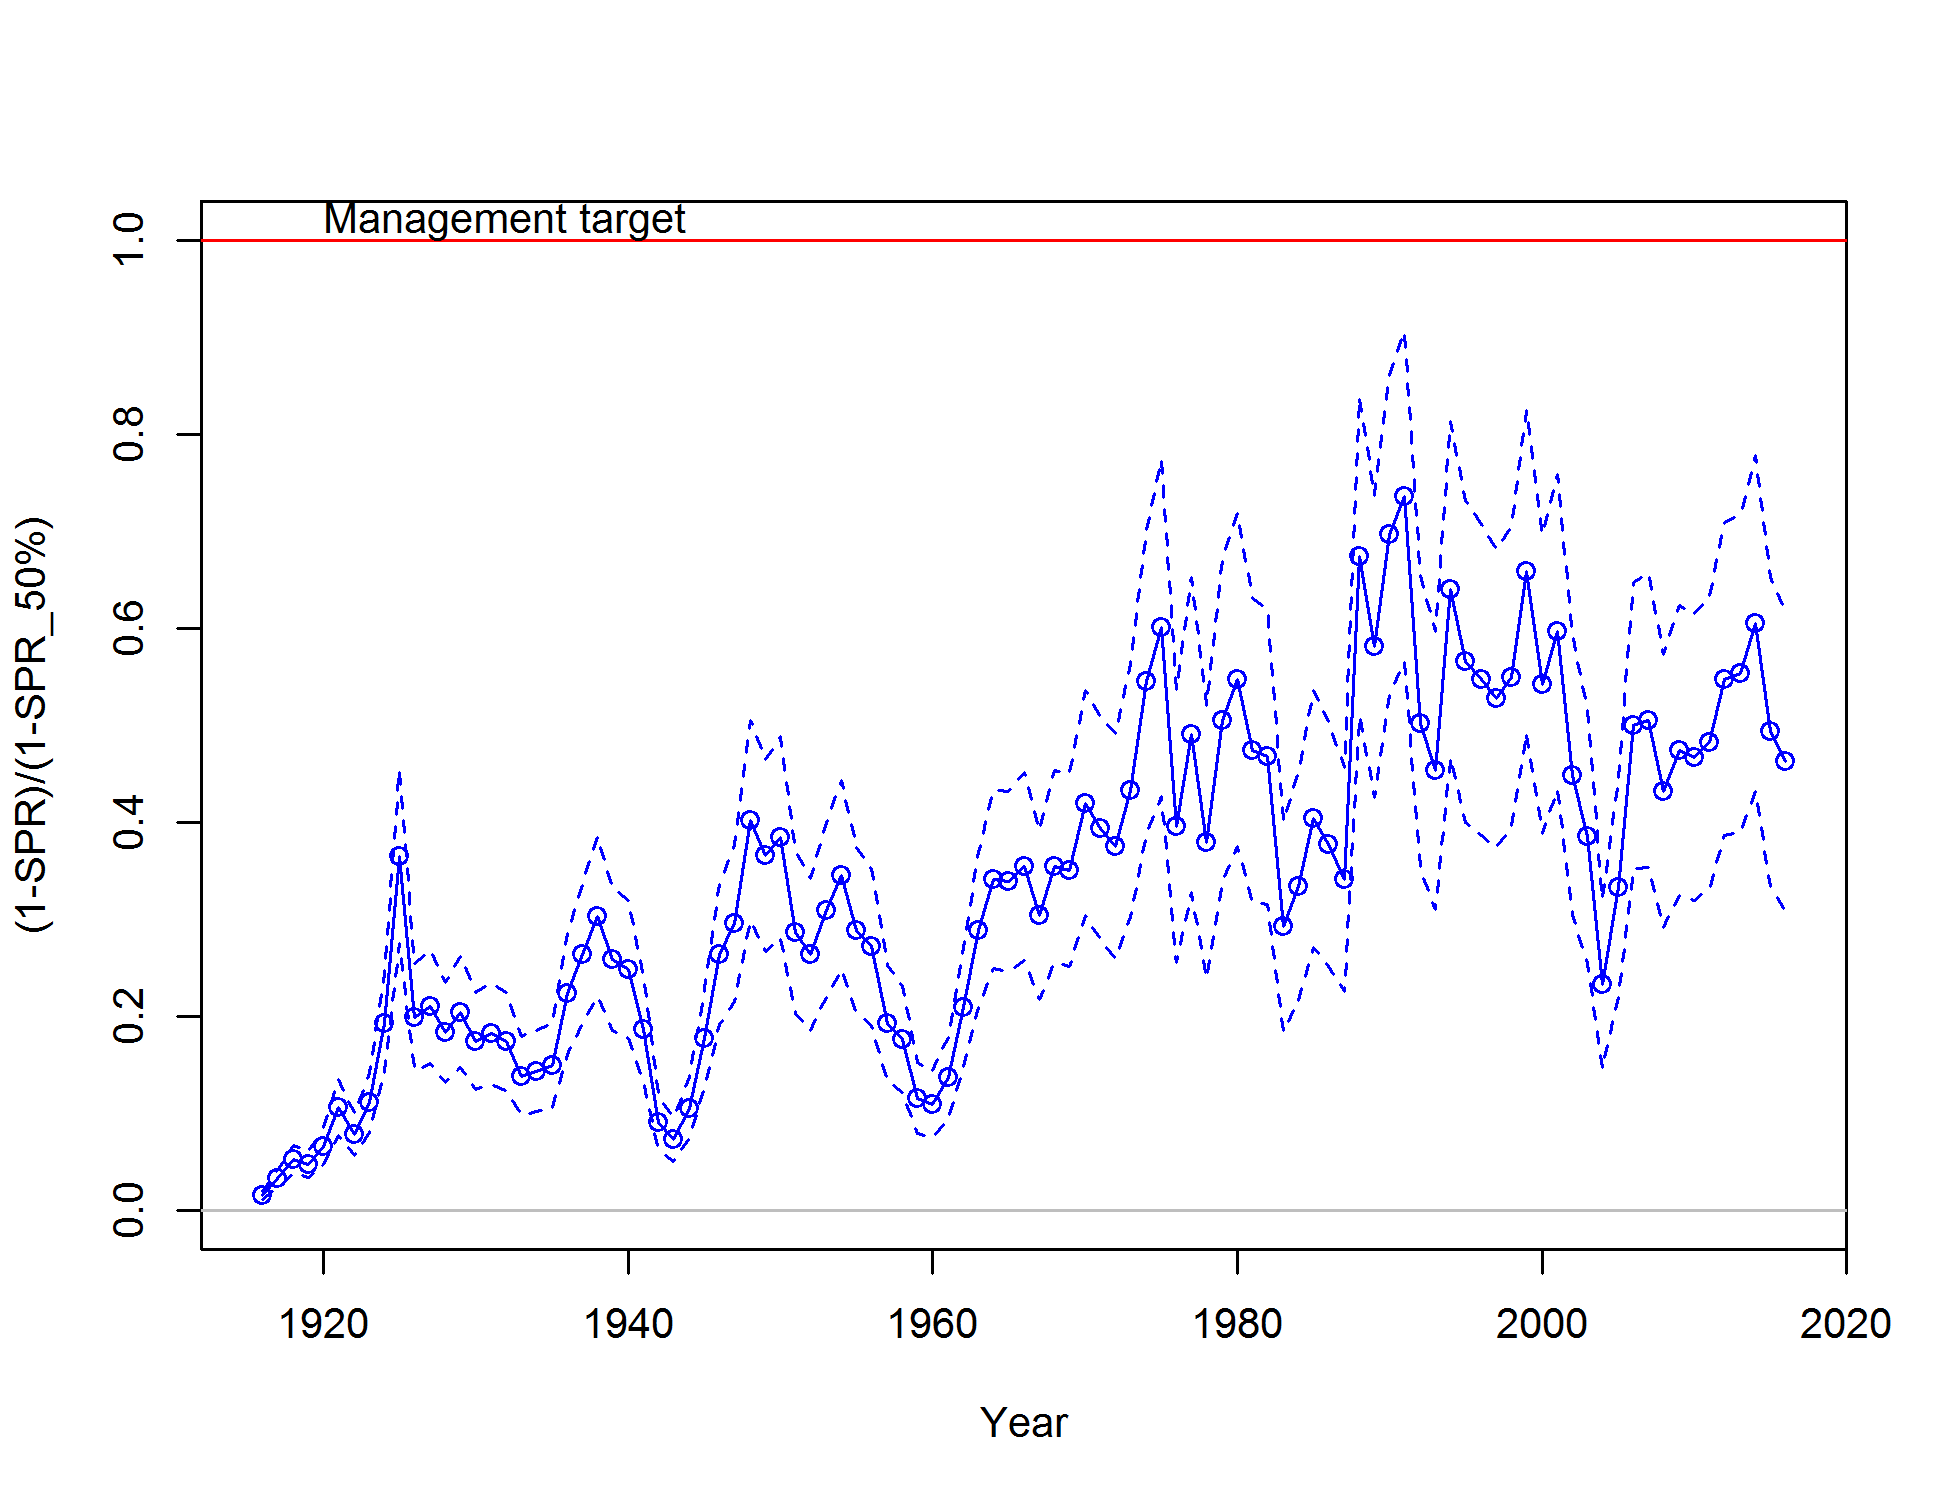
\includegraphics{r4ss/plots_mod1/SPR3_ratiointerval.png} \endcol
 \begincol{.5\textwidth}
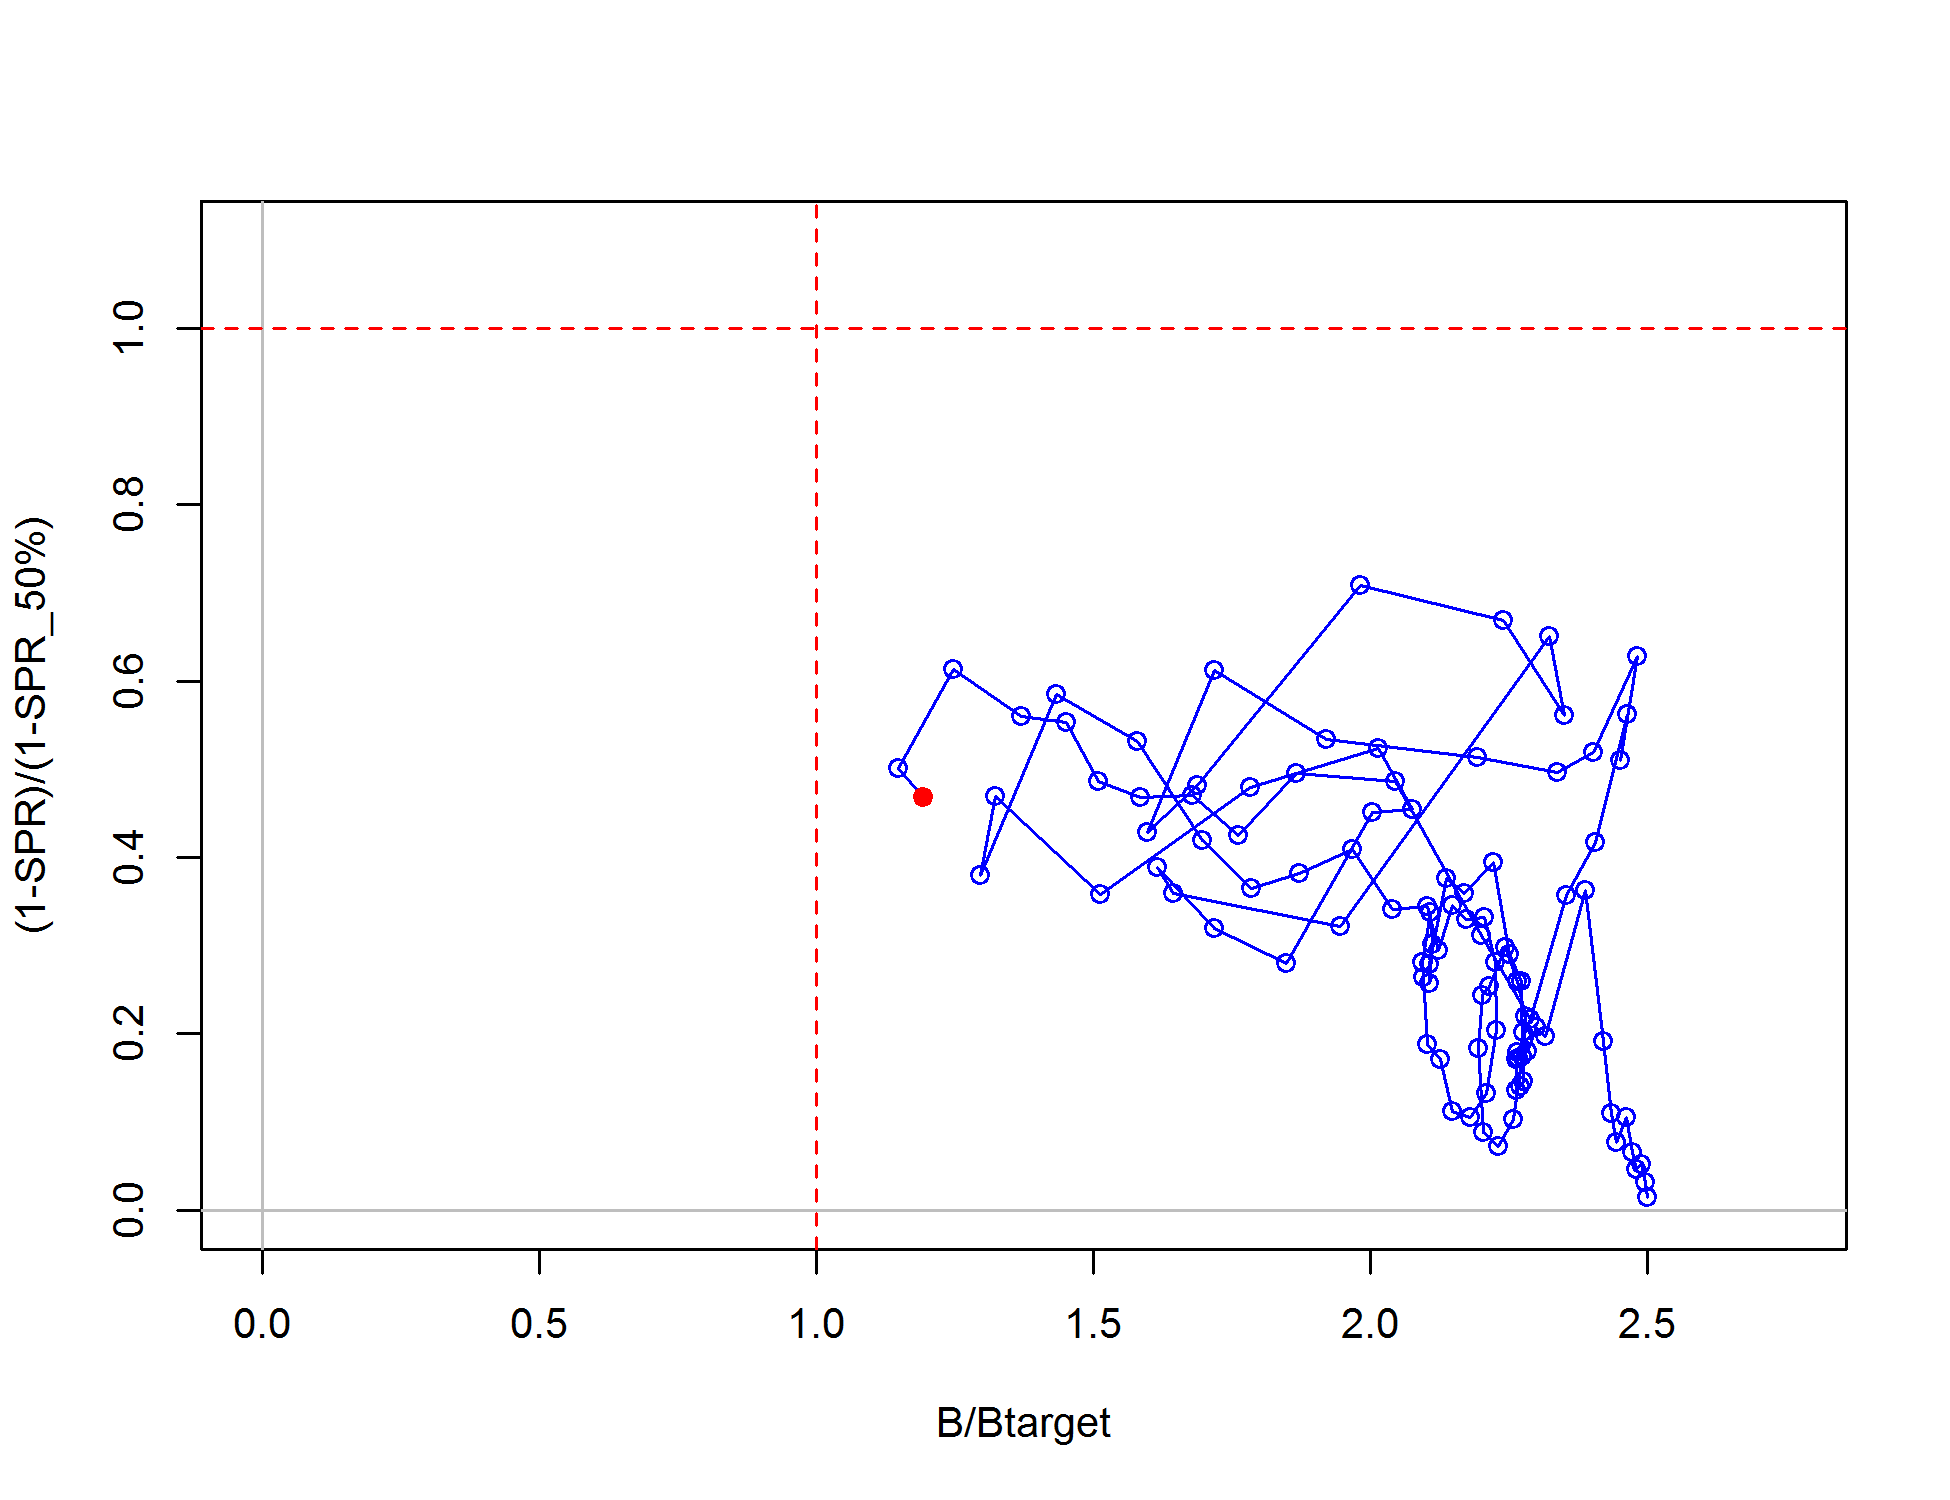
\includegraphics{r4ss/plots_mod1/SPR4_phase.png} \endcol
\endcols

\end{frame}

\begin{frame}{Stock Status - Eq. Yield}

\centering
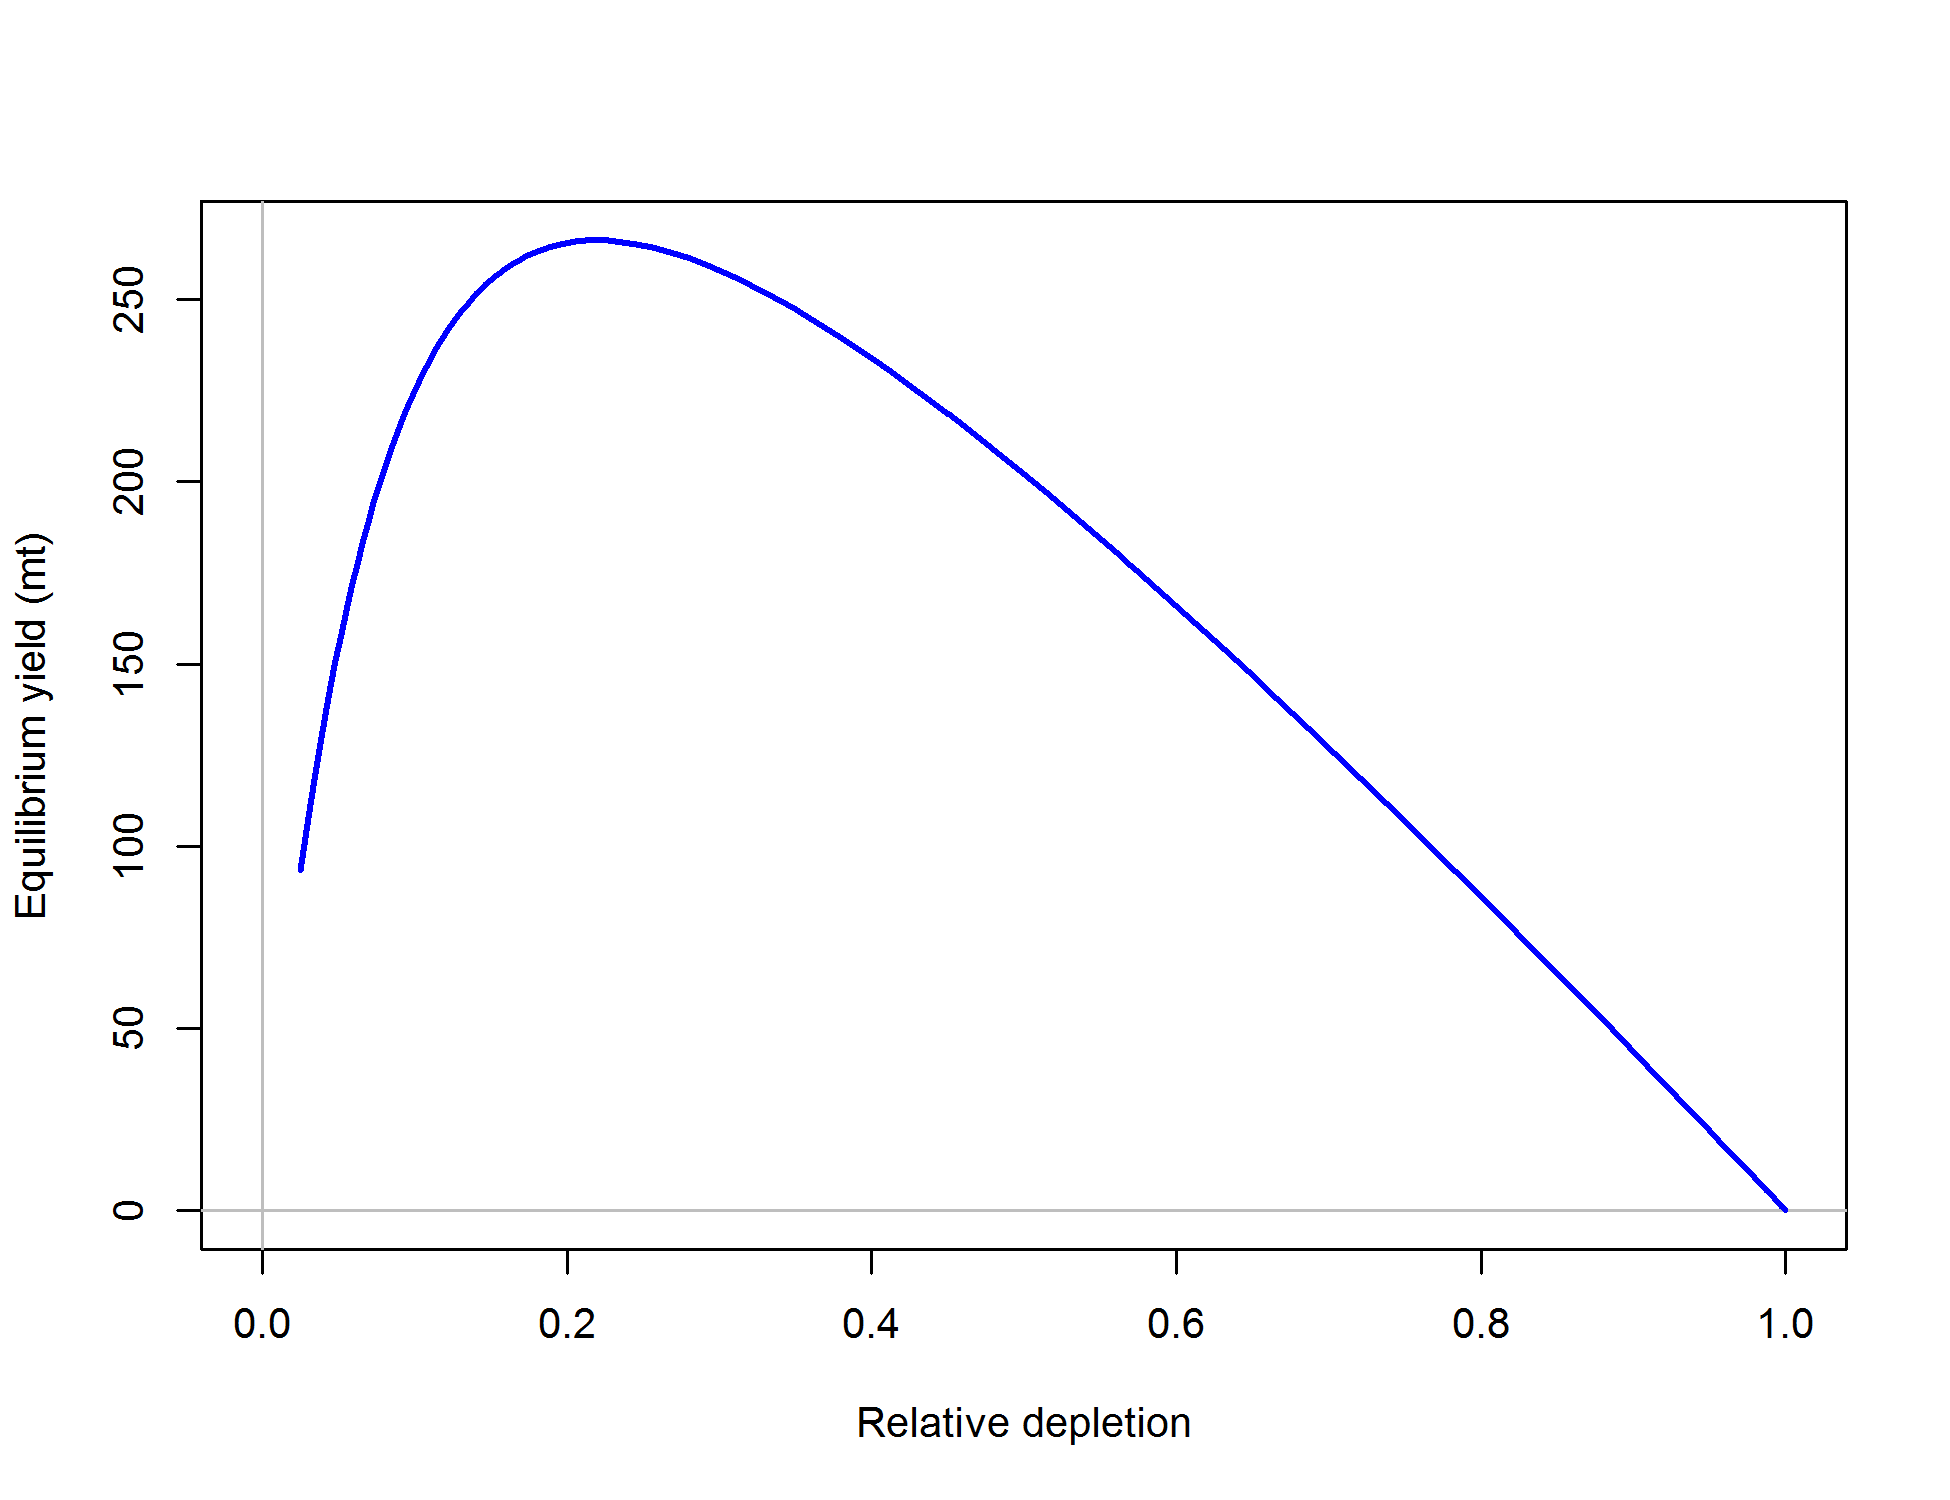
\includegraphics{r4ss/plots_mod1/yield1_yield_curve.png}

\end{frame}

\begin{frame}{Reference Points}

\begin{table}[ht]
\centering
\scalebox{0.7}{
\begin{tabular}{lll}
  \hline
\textbf{Quantity} & \textbf{Estimate} & \textbf{\~95\%  Confidence Interval} \\ 
  \hline
Unfished spawning biomass (mt) & 1624.4 & (1156.4-2092.5) \\ 
  Unfished age 1+ biomass (mt) & 2921.9 & (2052.8-3791.1) \\ 
  Unfished recruitment ($R_0$) & 3619.8 & (2518.6-4721) \\ 
  Spawning biomass (2017, mt) & 882.5 & (484.2-1280.7) \\ 
  Depletion (2017) & 0.5432 & (0.4299-0.6565) \\ 
  \textbf{$\text{Reference points based on } \mathbf{SB_{40\%}}$} &  &  \\ 
  Proxy spawning biomass ($B_{40\%}$) & 649.8 & (462.5-837) \\ 
  SPR resulting in $B_{40\%}$ ($SPR_{B40\%}$) & 0.4589 & (0.4589-0.4589) \\ 
  Exploitation rate resulting in $B_{40\%}$ & 0.1741 & (0.1601-0.1882) \\ 
  Yield with $SPR_{B40\%}$ at $B_{40\%}$ (mt) & 247.2 & (168.6-325.9) \\ 
  \textbf{\textit{Reference points based on SPR proxy for MSY}} &  &  \\ 
  Spawning biomass & 723.8 & (515.2-932.3) \\ 
  $SPR_{proxy}$ & 0.5 &  \\ 
  Exploitation rate corresponding to $SPR_{proxy}$ & 0.1502 & (0.1383-0.1621) \\ 
  Yield with $SPR_{proxy}$ at $SB_{SPR}$ (mt) & 232.4 & (158.5-306.4) \\ 
  \textbf{\textit{Reference points based on estimated MSY values}} &  &  \\ 
  Spawning biomass at $MSY$ ($SB_{MSY}$) & 358.8 & (250.6-467) \\ 
  $SPR_{MSY}$ & 0.2974 & (0.2857-0.3091) \\ 
  Exploitation rate at $MSY$ & 0.3236 & (0.2917-0.3554) \\ 
  $MSY$ (mt)  & 281.3 & (192.2-370.4) \\ 
   \hline
\end{tabular}
}
\end{table}

\end{frame}

\begin{frame}{Sensitivities - All}

\includegraphics{Figures/Sensitivity_All.pdf}

\end{frame}

\begin{frame}{Decision Table}

\begin{table}[ht]
\centering
\scalebox{0.45}{
\begin{tabular}{l|cc|>{\centering}p{.7in}c|>{\centering}p{.7in}c|>{\centering}p{.7in}c}
   \multicolumn{3}{c}{}  &  \multicolumn{2}{c}{} 
                               & \multicolumn{2}{c}{\textbf{States of nature}} 
                               & \multicolumn{2}{c}{} \\
  \multicolumn{3}{c}{}  &  \multicolumn{2}{c}{Low M 0.164} 
                               & \multicolumn{2}{c}{Base M 0.235} 
                               &  \multicolumn{2}{c}{High M 0.2745} \\
 \hline
 & Year & Catch & Spawning biomass & Depletion & Spawning biomass & Depletion & Spawning biomass & Depletion \\ 
  \hline
 & 2019 & 150.00 & 587.05 & 0.47 & 1154.73 & 0.71 & 2252.89 & 0.84 \\ 
   & 2020 & 150.00 & 584.87 & 0.47 & 1174.89 & 0.72 & 2312.02 & 0.86 \\ 
   & 2021 & 150.00 & 574.64 & 0.46 & 1176.29 & 0.72 & 2331.33 & 0.87 \\ 
  Constant & 2022 & 150.00 & 561.72 & 0.45 & 1169.09 & 0.72 & 2330.83 & 0.87 \\ 
  Catch & 2023 & 150.00 & 548.66 & 0.44 & 1158.79 & 0.71 & 2321.64 & 0.86 \\ 
   & 2024 & 150.00 & 536.43 & 0.43 & 1148.13 & 0.71 & 2309.70 & 0.86 \\ 
   & 2025 & 150.00 & 525.20 & 0.42 & 1138.24 & 0.70 & 2297.82 & 0.86 \\ 
   & 2026 & 150.00 & 514.89 & 0.41 & 1129.45 & 0.70 & 2287.10 & 0.85 \\ 
   & 2027 & 150.00 & 505.35 & 0.40 & 1121.77 & 0.69 & 2277.85 & 0.85 \\ 
   & 2028 & 150.00 & 496.46 & 0.40 & 1115.12 & 0.69 & 2270.05 & 0.85 \\ 
   \hline
 & 2019 & 232.40 & 573.15 & 0.46 & 984.92 & 0.61 & 1779.53 & 0.66 \\ 
   & 2020 & 232.40 & 588.87 & 0.47 & 955.43 & 0.59 & 1673.88 & 0.62 \\ 
   & 2021 & 232.40 & 592.42 & 0.47 & 912.16 & 0.56 & 1560.33 & 0.58 \\ 
  Estimated & 2022 & 232.40 & 588.94 & 0.47 & 869.23 & 0.54 & 1462.95 & 0.54 \\ 
  MSY & 2023 & 232.40 & 584.63 & 0.47 & 837.51 & 0.52 & 1400.62 & 0.52 \\ 
   & 2024 & 232.40 & 579.50 & 0.46 & 812.51 & 0.50 & 1353.76 & 0.50 \\ 
   & 2025 & 232.40 & 575.83 & 0.46 & 796.20 & 0.49 & 1327.05 & 0.49 \\ 
   & 2026 & 232.40 & 572.04 & 0.46 & 782.22 & 0.48 & 1302.32 & 0.48 \\ 
   & 2027 & 232.40 & 569.72 & 0.45 & 773.77 & 0.48 & 1290.11 & 0.48 \\ 
   & 2028 & 232.40 & 567.04 & 0.45 & 765.22 & 0.47 & 1275.09 & 0.47 \\ 
   \hline
 & 2019 & 346.30 & 587.05 & 0.47 & 1154.73 & 0.71 & 2252.89 & 0.84 \\ 
   & 2020 & 333.89 & 479.44 & 0.38 & 1068.32 & 0.66 & 2206.66 & 0.82 \\ 
   & 2021 & 313.01 & 383.32 & 0.31 & 983.88 & 0.61 & 2142.68 & 0.80 \\ 
  ACL = ABC & 2022 & 293.00 & 311.34 & 0.25 & 917.22 & 0.56 & 2085.85 & 0.78 \\ 
   & 2023 & 277.18 & 260.27 & 0.21 & 869.36 & 0.54 & 2042.74 & 0.76 \\ 
   & 2024 & 265.38 & 221.15 & 0.18 & 835.93 & 0.51 & 2012.49 & 0.75 \\ 
   & 2025 & 256.64 & 187.64 & 0.15 & 812.37 & 0.50 & 1992.23 & 0.74 \\ 
   & 2026 & 250.12 & 157.42 & 0.13 & 795.36 & 0.49 & 1979.19 & 0.74 \\ 
   & 2027 & 245.19 & 129.79 & 0.10 & 782.82 & 0.48 & 1971.20 & 0.73 \\ 
   & 2028 & 241.44 & 104.22 & 0.08 & 773.46 & 0.48 & 1966.69 & 0.73 \\ 
   \hline
\hline
\end{tabular}
}
\end{table}

\end{frame}

\begin{frame}{Research and Data Needs}

\begin{itemize}
\item[$\bullet$] \textbf{Natural mortality and steepness}: Both natural mortality and steepness were 
fixed in the base model.  The natural mortality estimate used the assessment 
was based on maximum age and steepness based on rockfish species meta-analysis.

\item[$\bullet$] \textbf{Stock south of the U.S. border}:  No available information on the status of California scorpionfish in Mexico could be found.

\item[$\bullet$] \textbf{Sex ratio}:  The sex ratio in the only published work by Love et al.
(\protect\hyperlink{ref-Love1987}{1987}) and samples 
from the NWFSC trawl survey were skewed towards males.

\item[$\bullet$] \textbf{Aggregating behavior}: Aggregative behavior in both spawning and 
non-spawning seasons of California scorpionfish is not well understood.

\end{itemize}

\end{frame}

\begin{frame}{Research and Data Needs}

\begin{itemize}

\item[$\bullet$] \textbf{Fecundity/maturity}: A reproductive biology study of California 
scorpionfish is needed.There are currently no estimates of fecundity 
for California scorpionfish and no studies have been done of the relationship between weight and reproductive 
output.

\item[$\bullet$] \textbf{Discard mortality}: Many scorpionfish are discarded at sea. The assessment 
used estimates of discard mortality of a distantly related species (lingcod) 
in a different ecological setting (Karpov \protect\hyperlink{ref-Karpov1996}{1996}). 


\item[$\bullet$] \textbf{Environmental covariates}: The relationship between environmental 
conditions and recruitment for scorpionfish should be further explored. Preliminary 
exploration using CalCOFI temperature data suggested that a relationship existed, 
but other time series may correlate more strongly given that scorpionfish are a 
near-shore species.

\end{itemize}

\end{frame}

\begin{frame}{Research and Data Needs}

\begin{itemize}

\item[$\bullet$] \textbf{Discard fleet modeling}: Modeling discard as a separate fleet, as 
was done for California scorpionfish, is a simple and intuitive approach, but 
the strengths and weaknesses of this approach are unclear.

\item[$\bullet$] \textbf{POTW trawl surveys}: Additional biological information 
(sex, otoliths, depth distribution) should be collected for California 
scorpionfish during the Publicly Owned Treatment Works (POTWs) trawl 
survey and the Southern California Bight Regional Monitoring Project 
(SCCWRP) trawl survey.

\item[$\bullet$] \textbf{Age validation}: An age validation study is needed for 
California scorpionfish.

\end{itemize}

\end{frame}

\begin{frame}{Questions??}

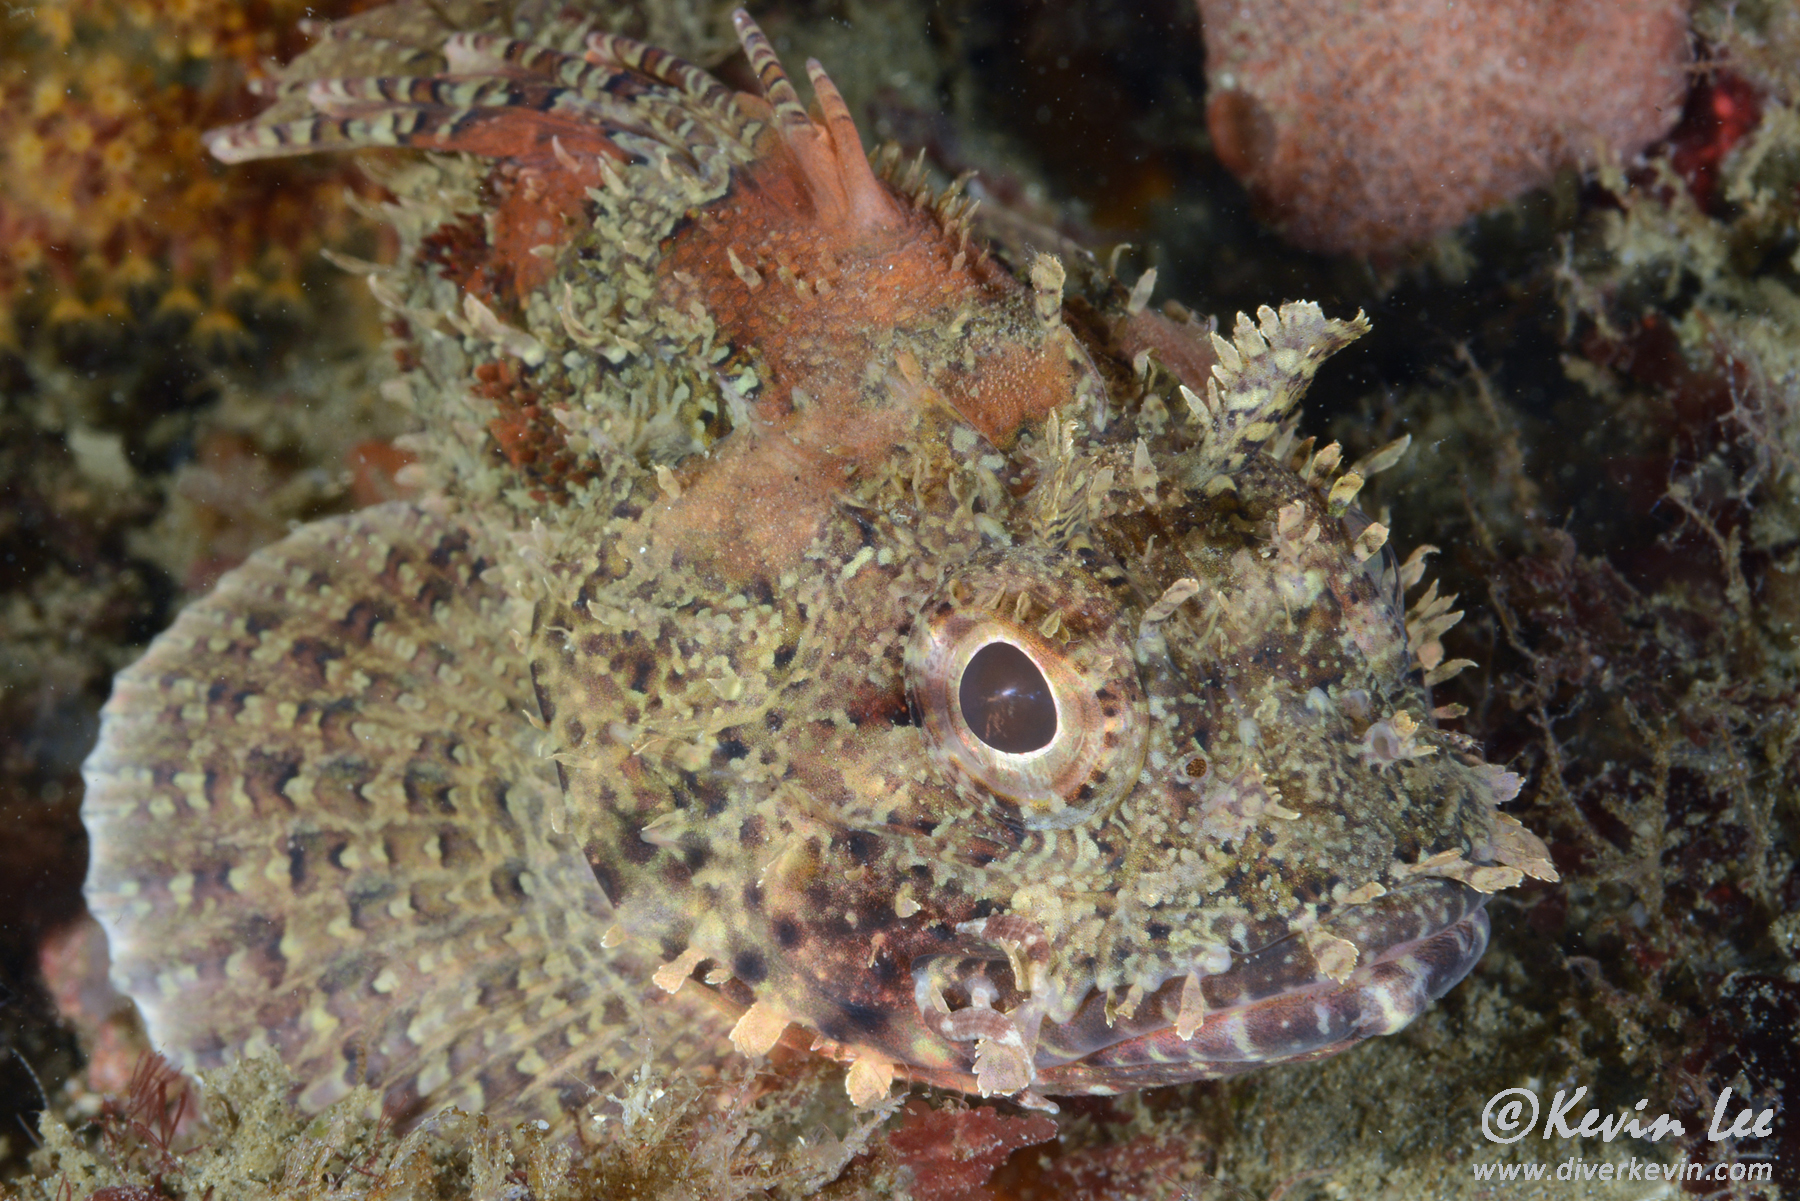
\includegraphics[width=\textwidth]{cover_photo}

\end{frame}

\begin{frame}{Uncertainties Identified by the STAR panel}

\begin{itemize}
\item[$\bullet$] The stock likely extends south of southern boundary of the assessment at the US/Mexico border.  
\item[$\bullet$] Maturity estimates used are dated and cannot be reproduced.  No studies have been done of the relationship between fish weight and reproductive output.
\item[$\bullet$] Ageing samples come only from the NWFSC shelf-slope survey NW slope shelf survey ($\geq 55 m$) and thus does not cover the depth distribution of the stock.  The maximum age from this data set could be biased. 
\item[$\bullet$] Estimates of discard mortality based of a distantly related species (lingcod) in a different ecological setting.
\item[$\bullet$] Steepness in the assessment was based on the Thorson prior, which is only strictly appropriate for West Coast rockfish (\emph{Sebastes} spp.). 
\end{itemize}

\end{frame}

\end{document}
